\chapter{概率分布的逼近}
\label{chap:distribution-approximation}

实数轴上有一个分布，我们只知道它的密度正比于
\[
 \widetilde{\pi}(x)=\mathrm{e}^{-x^{4}/4} .
\]
任给一个$x$，$\widetilde{\pi}(x)$都能立即算出；可是要回答“$X$落在$[-1,1]$外的概率是多少”“$X^{2}$的平均是多少”，就要先求归一化常数$\int\widetilde{\pi}\,\mathrm{d}x$，再做积分。一维时数值积分不难，若变量有几十个分量，同样的积分就无法逐格计算。一个自然的想法是找一个容易计算的分布，比如某个高斯分布，代替它回答这些问题。

这样做立刻带来四个问题。第一，候选分布从哪里选：所有高斯分布，所有各分量独立的分布，还是某个有限维参数族？候选集合定下以后，有些性质无论怎样选都保留不下来。第二，“最接近”按什么标准：第~\ref{chap:distribution-comparison}章的KL散度有两个方向，分别按候选分布和按目标分布加权，选出的分布一般不同。第三，怎样求出最接近的候选：有时能逐个因子写出最优更新，有时只能对参数做梯度下降。第四，得到的近似有多好：误差既来自候选集合的表达能力，也来自没有算到最优，还来自期望的数值计算。

本章依次回答这四个问题。第一节固定目标分布，区分候选分布能计算密度、能抽样和能求期望这几项不同的要求，并用两个变量的概率表说明结构限制怎样删去依赖。第二节分别研究两个方向的KL目标，说明各自的支持条件、权重与计算需求，并在一个三点分布的例子中算出两个方向的最优解。第三节把候选限制为乘积分布，先在相关高斯分布上看独立性限制改变了哪些数值特征，再推导逐因子的坐标更新。第四节处理有限维参数族上的梯度更新。第五节把误差分成几个来源，说明怎样按任务检验近似结果。

本章回用第~\ref{chap:distribution-families}章的分布族，特别是指数族的对数配分函数与均值参数；第~\ref{chap:distribution-comparison}章的KL散度、Gibbs不等式与Pinsker不等式；第~\ref{chap:information-measures}章的交叉熵与互信息。上一章在满足约束的全体分布中选择分布，那里的最优解由问题本身给出；本章的目标分布已经给定，困难在于候选集合受到限制。

\section{目标分布与候选族}
\label{sec:dapx-target-candidates}

逼近问题有两个输入：要逼近的分布，以及允许用来逼近的分布。前者在本章中始终固定，后者由我们选择。选择候选集合时，首先要弄清“容易计算”具体指哪几种计算，其次要弄清限制候选集合会丢掉什么，最后要检查逼近目标对这两个集合是否有定义。

\paragraph{目标分布}
设取值空间$\mathcal{X}$上有一个概率分布$\Pi$，称为\term{目标分布}（target distribution）。取一个参考测度$\lambda$：有限或可数的$\mathcal{X}$上取计数测度，$\mathbb{R}^{d}$上取Lebesgue测度。设$\Pi\ll\lambda$，密度记为$\pi$。很多时候我们只知道
\begin{equation}
 \pi(x)=\frac{\widetilde{\pi}(x)}{Z},\qquad Z=\int_{\mathcal{X}}\widetilde{\pi}\,\mathrm{d}\lambda,\qquad 0<Z<\infty ,
 \label{eq:dapx-unnormalized}
\end{equation}
其中$\widetilde{\pi}\geq0$可以逐点计算，称为\term{未归一化密度}（unnormalized density），而$Z$算不出来。条件$0<Z<\infty$保证$\Pi$是一个合法的概率分布；它是逼近问题的前提，不是逼近要解决的问题。

计算困难通常来自维数。设$\bm{x}=(x_1,\dots,x_m)\in\{0,1\}^{m}$，未归一化密度由成对的相互作用给出，
\[
 \widetilde{\pi}(\bm{x})=\exp\Bigl(\sum_{i<j}J_{i,j}x_ix_j+\sum_{i}h_ix_i\Bigr) .
\]
任给一个$\bm{x}$，计算$\widetilde{\pi}(\bm{x})$只需要做$m(m-1)/2+m$次乘加。$Z$却是$2^{m}$项之和，$m=50$时约$10^{15}$项；边缘概率$\Pi(X_1=1)$也要对其余$49$个分量的$2^{49}$种取值求和。密度可以逐点算，却不等于概率和期望可以算。

\paragraph{候选集合与三种计算}
用来逼近的分布组成\term{候选集合}（candidate set）$\mathcal{Q}$，其中每个$Q$也对$\lambda$有密度$q$。第~\ref{chap:distribution-families}章给出了构造候选集合的几种方式：有限维参数族$\{q_{\bm{\theta}}:\bm{\theta}\in\Theta\}$、指数族、混合分布、由简单随机变量经变换得到的推前族。选哪一种，要看后面需要对候选分布做哪些计算。这些计算可以分成三项：
\begin{itemize}
 \item \textbf{计算密度}：任给$x$，算出$q(x)$或$\ln q(x)$，有时允许差一个常数；
 \item \textbf{抽样}：生成服从$Q$的独立样本；
 \item \textbf{求期望}：对给定的函数$f$，算出$\mathbb{E}_{Q}[f(X)]$的准确值或足够准确的近似。
\end{itemize}
三项能力相互独立，有一项不代表有另一项。表~\ref{tab:dapx-abilities}列出几类常见分布的情况。

\begin{BookInlineTable}
 \centering
 \caption{几类分布在三项计算上的情况。“是”指有闭式或可以直接执行的算法；求期望一栏针对后文常用的$\mathbb{E}[\ln q(X)]$与低次多项式的期望。}
 \label{tab:dapx-abilities}
 \begin{tabular}{llll}
  \toprule
  分布 & 密度 & 抽样 & 期望\\
  \midrule
  高斯分布 & 是 & 是 & 是\\
  有限状态乘积 & 是 & 是 & 逐因子求和\\
  高斯混合 & 是 & 是 & $\ln q$的期望无闭式\\
  推前族$X=g(Z)$ & 需可逆换元 & 是 & 借助样本\\
  未归一化目标 & 差常数$Z$ & 一般不能 & 一般不能\\
  \bottomrule
 \end{tabular}
\end{BookInlineTable}

高斯混合的密度是几个高斯密度的加权和，可以逐点计算，抽样也只需先抽成分再抽高斯；但$\ln q$是和的对数，它在$Q$下的期望没有闭式，只能数值计算。推前族由$X=g(Z)$定义，$Z$容易抽样，于是$X$也容易抽样；可是$X$的密度要用换元公式，需要$g$可逆、可微并能算Jacobian行列式，否则密度可能根本不存在（第~\ref{chap:distribution-families}章中，$g$把低维的随机变量送进高维空间时，输出落在一个零测集上，就没有密度）。所以，“有一个解析的密度表达式”或“能抽样”都不能代表后续所有计算都已可行，必须对照逼近目标实际需要的计算逐项核对。

\paragraph{结构限制删去依赖}
候选集合的限制不只是“分布形状更简单”，还可能直接删去目标中的某种关系。取两个二值变量，目标分布由概率表给出：
\begin{equation}
 \pi(0,0)=\pi(1,1)=0.45,\qquad \pi(0,1)=\pi(1,0)=0.05 .
 \label{eq:dapx-table}
\end{equation}
两个变量各自取$0$和$1$的概率都是$\tfrac12$，但它们几乎总是相等：$\Pi(X_1=X_2)=0.9$。现在只允许用乘积分布$q(x_1,x_2)=q_1(x_1)q_2(x_2)$逼近它，即$X_1,X_2$在候选分布下独立。记$a=q_1(1)$，$b=q_2(1)$，则
\[
 Q(X_1=X_2)=(1-a)(1-b)+ab .
\]

若要求候选保留目标的两个边缘，必须$a=b=\tfrac12$，此时$Q(X_1=X_2)=\tfrac12$，远小于$0.9$。若要让$Q(X_1=X_2)$接近$0.9$，就要把$a,b$同时推向$0$或同时推向$1$，边缘又不再是$\tfrac12$。乘积候选不能同时保留两个边缘和“两个变量常常相等”这一事实，无论怎样选择$a,b$都是如此。图~\ref{fig:dapx-table-product}画出目标表和它的边缘乘积：对角线上的集中完全消失了。

\begin{BookInlineFigure}
 \centering
 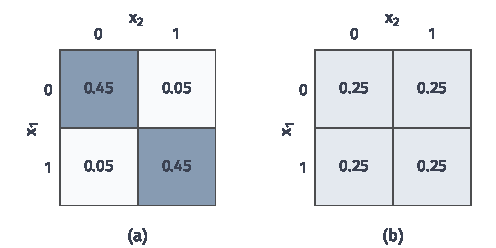
\includegraphics[width=84mm]{figures/07-probability/07-distribution-optimization/matplotlib/dapx-table-product/figure.pdf}
 \caption{结构限制删去依赖。(a)式~\eqref{eq:dapx-table}的目标概率表，行是$x_1$，列是$x_2$，颜色越深概率越大。(b)它的两个边缘都是$(\tfrac12,\tfrac12)$，边缘乘积在四格上都是$0.25$。}
 \label{fig:dapx-table-product}
\end{BookInlineFigure}

这里丢掉的东西可以用第~\ref{chap:information-measures}章的互信息度量。目标与它的边缘乘积之间的KL散度就是$I(X_1;X_2)$，计算得
\[
 D_{\mathrm{KL}}(\Pi\Vert\Pi_1\otimes\Pi_2)=0.9\ln\frac{0.45}{0.25}+0.1\ln\frac{0.05}{0.25}=0.9\ln1.8-0.1\ln5\approx0.3681 .
\]
第~\ref{sec:dapx-mean-field}节将证明，在按目标加权的方向上，这个数恰好是乘积候选所能达到的最小KL；在另一个方向上，最优的乘积分布并不是边缘乘积。

\paragraph{支持、参数范围与可积性}
选定候选集合后，还要检查逼近目标在这两个集合之间是否有意义。第一项检查是支持。设目标是$\operatorname{Exp}(1)$，密度在$x<0$处为零，候选集合是全体一维高斯分布。每个高斯分布都给$(-\infty,0)$正概率，所以$Q\ll\Pi$不成立；按第~\ref{chap:distribution-comparison}章的约定，$D_{\mathrm{KL}}(Q\Vert\Pi)=+\infty$对每个候选成立，这个方向的KL无法区分任何两个候选。另一个方向$D_{\mathrm{KL}}(\Pi\Vert Q)$则对每个高斯候选有限，因为高斯密度处处为正。图~\ref{fig:dapx-support}(a)中红色区域就是候选有质量而目标没有的部分。

第二项检查是参数范围。参数必须落在使候选成为合法分布的集合内：标准差为正，概率表的分量非负且和为$1$，协方差矩阵对称正定，混合权重在单纯形上。优化时这些都是约束，第~\ref{sec:dapx-gradient}节会用重新参数化来自动满足它们。

第三项检查是可积性。绝对连续只保证对数比几乎处处有限，不保证它的期望有限。取目标为标准Cauchy分布，候选为$\mathcal{N}(0,1)$。两个密度处处为正，但
\[
 \ln\frac{\pi(x)}{q(x)}=\frac{x^{2}}{2}-\ln(1+x^{2})+\ln\sqrt{\frac{2}{\pi}} ,
\]
它在Cauchy分布下的期望含有$\mathbb{E}_{\Pi}[X^{2}]=+\infty$，所以$D_{\mathrm{KL}}(\Pi\Vert Q)=+\infty$。把$\mathcal{N}(0,1)$换成任何其他高斯分布，对数比中仍有$x^{2}$的正系数项，结论不变：这个方向对全体高斯候选都是无穷大。反方向的被积函数在高斯权重下迅速衰减，$D_{\mathrm{KL}}(Q\Vert\Pi)$有限，数值积分给出约$0.259$。

\begin{BookInlineFigure}
 \centering
 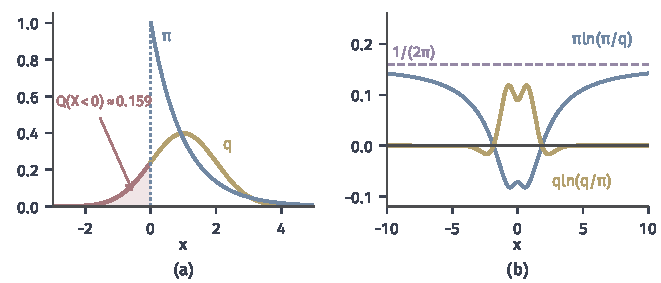
\includegraphics[width=112mm]{figures/07-probability/07-distribution-optimization/matplotlib/dapx-support/figure.pdf}
 \caption{逼近目标可能对所有候选都无穷大。(a)目标$\operatorname{Exp}(1)$（蓝）与候选$\mathcal{N}(1,1)$（黄），红色区域是候选落在$x<0$的质量$\Phi(-1)\approx0.159$，目标在那里没有质量，所以$D_{\mathrm{KL}}(Q\Vert\Pi)=+\infty$。(b)目标为标准Cauchy分布、候选为$\mathcal{N}(0,1)$时两个方向的被积函数：蓝线$\pi\ln(\pi/q)$在远处趋于常数$1/(2\pi)$（紫色虚线），积分发散；黄线$q\ln(q/\pi)$迅速衰减。}
 \label{fig:dapx-support}
\end{BookInlineFigure}

图~\ref{fig:dapx-support}(b)显示了无穷大的来源：Cauchy分布在远处的密度约为$1/(\pi x^{2})$，乘上对数比中的$x^{2}/2$后趋于常数$1/(2\pi)$，在整条直线上积分必然发散。这两个例子说明，KL目标是否有限取决于目标、候选与方向三者的组合。确定候选集合时就要检查它，不能留到优化出问题时再发现。

\section{逼近目标}
\label{sec:dapx-objectives}

候选集合定下以后，要从中挑一个“离目标最近”的分布。第~\ref{chap:distribution-comparison}章给了许多比较分布的量，本章以KL散度为主，因为它的对数比可以按候选分布或目标分布逐点平均，后面的坐标更新和梯度更新都由此推出。KL散度不对称，于是有两个逼近问题：
\begin{equation}
 \min_{Q\in\mathcal{Q}}D_{\mathrm{KL}}(Q\Vert\Pi),\qquad \min_{Q\in\mathcal{Q}}D_{\mathrm{KL}}(\Pi\Vert Q) .
 \label{eq:dapx-two-problems}
\end{equation}
前者的期望按候选分布$Q$计算，后者按目标分布$\Pi$计算。用来做平均的分布不同，带来三处差别：误差在哪里被计入，KL有限需要什么支持条件，计算时需要能对哪个分布求期望。

先说明本节结论的范围。KL散度只是一种比较量。若后续任务关心的是某个事件的概率、某个矩或某个距离，应当按第~\ref{chap:distribution-comparison}章的方法对相应的量另行检查，第~\ref{sec:dapx-error}节会做这样的检查。使某个KL最小的候选，并不自动使其他比较量也最小。

\subsection{按候选分布计算KL}
\label{sec:dapx-reverse-kl}

第一个问题是
\begin{equation}
 \min_{Q\in\mathcal{Q}}D_{\mathrm{KL}}(Q\Vert\Pi)=\min_{Q\in\mathcal{Q}}\mathbb{E}_{Q}\Bigl[\ln\frac{q(X)}{\pi(X)}\Bigr] .
 \label{eq:dapx-reverse-problem}
\end{equation}
它在文献中常称为\term{反向KL散度}（reverse KL divergence）的最小化，“反向”是相对于下一小节按目标加权的方向而言。

\paragraph{误差按候选分布计入}
被积函数$q\ln(q/\pi)$只在候选有质量的地方才有分量。候选给某处很高的概率而目标在那里概率很小，对数比$\ln(q/\pi)$很大，又乘以较大的权重$q$，代价很重。反过来，目标在某处有质量而候选在那里几乎没有质量，权重$q$接近零，这一处几乎不计入。所以这个方向主要惩罚“候选在目标稀少的地方放了质量”，而对“候选漏掉了目标的一部分”宽容得多。

\paragraph{有限的条件}
由第~\ref{chap:distribution-comparison}章的定义，$D_{\mathrm{KL}}(Q\Vert\Pi)<\infty$首先要求$Q\ll\Pi$：候选不能把正概率放在目标概率为零的集合上。上一节的$\operatorname{Exp}(1)$目标与高斯候选就违反这一条。其次，对数比的负部总是可积的，所以在$Q\ll\Pi$时，KL有限当且仅当$\ln(q/\pi)$的正部在$Q$下可积。

\paragraph{未归一化目标}
目标只以式~\eqref{eq:dapx-unnormalized}的形式给出时，把$\pi=\widetilde{\pi}/Z$代入对数比：
\[
 \ln\frac{q(x)}{\pi(x)}=\ln q(x)-\ln\widetilde{\pi}(x)+\ln Z .
\]
$\ln Z$是与$x$和$Q$都无关的常数。设$\ln q-\ln\widetilde{\pi}$在$Q$下可积，记
\begin{equation}
 J(Q)=\mathbb{E}_{Q}\bigl[\ln q(X)-\ln\widetilde{\pi}(X)\bigr] .
 \label{eq:dapx-J}
\end{equation}
对上式取$Q$下的期望，就得到
\begin{equation}
 D_{\mathrm{KL}}(Q\Vert\Pi)=J(Q)+\ln Z .
 \label{eq:dapx-J-shift}
\end{equation}

式~\eqref{eq:dapx-J-shift}有三个推论。第一，在候选集合上最小化$J$与最小化$D_{\mathrm{KL}}(Q\Vert\Pi)$得到同一个最优解，而计算$J$只需要逐点算$\widetilde{\pi}$并对$Q$求期望，不需要$Z$。第二，由KL非负，对每个候选都有
\begin{equation}
 \ln Z\geq-J(Q) ,
 \label{eq:dapx-lower-bound}
\end{equation}
等号当且仅当$Q=\Pi$。$-J(Q)$称为$\ln Z$的\term{变分下界}（variational lower bound），在候选集合中把$J$压得越低，这个下界就越紧。第三，$J$的数值本身不是KL：不知道$\ln Z$，就只知道两个候选的KL之差$J(Q)-J(Q')$，不知道任何一个候选离目标有多远。以优化求近似分布的做法统称为\term{变分逼近}（variational approximation），这里的“变分”指在一族分布中变动以求最优。

\paragraph{四次方目标}
回到章首的目标$\widetilde{\pi}(x)=\mathrm{e}^{-x^{4}/4}$，取候选$Q=\mathcal{N}(m,s^{2})$。式~\eqref{eq:dapx-J}的两项分别是高斯分布的负熵与四次矩：
\[
 \mathbb{E}_{Q}[\ln q(X)]=-\ln s-C,\qquad C=\tfrac12\ln(2\pi\mathrm{e})\approx1.4189 ,
\]
\[
 \mathbb{E}_{Q}[-\ln\widetilde{\pi}(X)]=\tfrac14\mathbb{E}_{Q}[X^{4}]=\tfrac14\bigl(m^{4}+6m^{2}s^{2}+3s^{4}\bigr) .
\]
第二式用了$X=m+sY$、$Y\sim\mathcal{N}(0,1)$，以及$\mathbb{E}[Y]=\mathbb{E}[Y^{3}]=0$、$\mathbb{E}[Y^{2}]=1$、$\mathbb{E}[Y^{4}]=3$。两式相加，
\begin{equation}
 J(m,s)=-\ln s-C+\tfrac14\bigl(m^{4}+6m^{2}s^{2}+3s^{4}\bigr) .
 \label{eq:dapx-quartic-J}
\end{equation}

$m$只出现在非负项$m^{4}+6m^{2}s^{2}$中，所以对每个$s$，$m=0$最好。令$m=0$，对$s$求导并令其为零：
\[
 -\frac1s+3s^{3}=0,\qquad s^{4}=\frac13 .
\]
于是最优候选是
\[
 s^{*}=3^{-1/4}\approx0.7598,\qquad (s^{*})^{2}=3^{-1/2}\approx0.5774 .
\]
代回式~\eqref{eq:dapx-quartic-J}，最小值为
\[
 J^{*}=\tfrac14\ln3-C+\tfrac14\approx0.2747-1.4189+0.25=-0.8943 .
\]
由式~\eqref{eq:dapx-lower-bound}，$\ln Z\geq0.8943$。

这个例子里$Z$恰好能算出来，可以核对。代换$u=x^{4}/4$给出
\[
 Z=2\int_{0}^{\infty}\mathrm{e}^{-x^{4}/4}\,\mathrm{d}x=2\cdot4^{-3/4}\,\Gamma\bigl(\tfrac14\bigr)\approx2.5637,\qquad \ln Z\approx0.9414 .
\]
所以最优高斯候选的KL是
\[
 D_{\mathrm{KL}}(Q^{*}\Vert\Pi)=J^{*}+\ln Z\approx0.0472 .
\]
下界$0.8943$与真值$0.9414$相差$0.0472$，正是这个KL。图~\ref{fig:dapx-unnormalized}(b)中，$J(Q_s)$与$D_{\mathrm{KL}}(Q_s\Vert\Pi)$是上下平移$\ln Z$的两条曲线，最低点在同一个$s$。

\begin{BookInlineFigure}
 \centering
 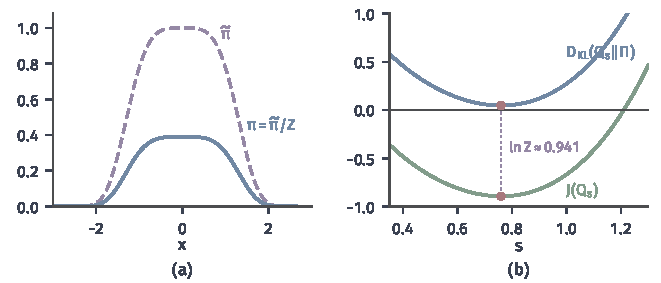
\includegraphics[width=112mm]{figures/07-probability/07-distribution-optimization/matplotlib/dapx-unnormalized/figure.pdf}
 \caption{未归一化目标。(a)$\widetilde{\pi}(x)=\mathrm{e}^{-x^{4}/4}$（紫色虚线）与归一化后的密度$\pi=\widetilde{\pi}/Z$（蓝），$Z\approx2.564$。(b)候选$Q_s=\mathcal{N}(0,s^{2})$：绿线是可计算的$J(Q_s)$，蓝线是$D_{\mathrm{KL}}(Q_s\Vert\Pi)$，两者相差常数$\ln Z\approx0.941$（紫色点线），在同一个$s^{*}=3^{-1/4}\approx0.760$处取最小值（红点）。}
 \label{fig:dapx-unnormalized}
\end{BookInlineFigure}

\paragraph{计算需求}
求$J(Q)$需要对候选$Q$求两个期望：$\ln q$与$\ln\widetilde{\pi}$。前者对高斯、乘积等候选通常有闭式；后者在本例中有闭式，一般情况下可以从$Q$抽样后取平均来估计，误差由第~\ref{chap:monte-carlo-integration-error}章分析。对目标$\Pi$只需要逐点计算$\widetilde{\pi}$，不需要$Z$，不需要从$\Pi$抽样，也不需要任何$\Pi$下的期望。这正是这个方向在目标难以计算时最常用的原因。

\subsection{按目标分布计算KL}
\label{sec:dapx-forward-kl}

第二个问题是
\begin{equation}
 \min_{Q\in\mathcal{Q}}D_{\mathrm{KL}}(\Pi\Vert Q)=\min_{Q\in\mathcal{Q}}\mathbb{E}_{\Pi}\Bigl[\ln\frac{\pi(X)}{q(X)}\Bigr] ,
 \label{eq:dapx-forward-problem}
\end{equation}
相应地常称为\term{正向KL散度}（forward KL divergence）的最小化。现在权重是$\pi$：目标常出现的地方，候选给的概率若太小就要付出代价。

\paragraph{有限的条件}
$D_{\mathrm{KL}}(\Pi\Vert Q)<\infty$要求$\Pi\ll Q$：候选必须覆盖目标有正概率的每个区域。只要漏掉一个这样的区域，KL就是$+\infty$。即使没有完全漏掉，覆盖不足也代价很重。取双峰目标
\begin{equation}
 \pi=0.7\,\mathcal{N}(-2,0.6^{2})+0.3\,\mathcal{N}(2,0.6^{2}) ,
 \label{eq:dapx-bimodal}
\end{equation}
候选$Q=\mathcal{N}(-2,0.6^{2})$只盖住左峰。数值积分给出
\[
 D_{\mathrm{KL}}(Q\Vert\Pi)\approx0.356,\qquad D_{\mathrm{KL}}(\Pi\Vert Q)\approx6.06 .
\]
按候选加权时，候选只看见左峰，在那里它的密度约是目标的$1/0.7$倍，代价约为$-\ln0.7\approx0.357$；按目标加权时，右峰有$0.3$的目标质量落在候选密度只有$\mathrm{e}^{-22}$量级的地方，峰顶处的对数比约为$21$，贡献了绝大部分代价。图~\ref{fig:dapx-weighting}(b)画出两个被积函数。

\begin{BookInlineFigure}
 \centering
 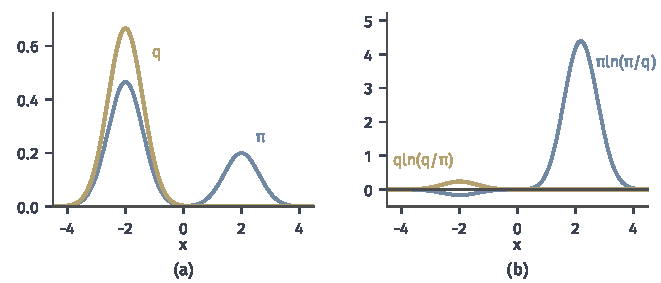
\includegraphics[width=112mm]{figures/07-probability/07-distribution-optimization/matplotlib/dapx-weighting/figure.pdf}
 \caption{两个方向的误差权重。(a)式~\eqref{eq:dapx-bimodal}的双峰目标（蓝）与只覆盖左峰的候选$\mathcal{N}(-2,0.6^{2})$（黄）。(b)被积函数：黄线$q\ln(q/\pi)$只在左峰附近有一个小鼓包，积分约$0.356$；蓝线$\pi\ln(\pi/q)$在右峰处高达$4$以上，积分约$6.06$。}
 \label{fig:dapx-weighting}
\end{BookInlineFigure}

\paragraph{与交叉熵的关系}
在离散情形，第~\ref{chap:information-measures}章已经证明，$H(\Pi)<\infty$时
\[
 D_{\mathrm{KL}}(\Pi\Vert Q)=H(\Pi,Q)-H(\Pi) .
\]
对一般的参考测度，同样的拆分需要两个积分分别有限：设$\mathbb{E}_{\Pi}\lvert\ln\pi(X)\rvert<\infty$与$\mathbb{E}_{\Pi}\lvert\ln q(X)\rvert<\infty$，则可以把对数比的期望拆成两项之差，
\begin{equation}
 D_{\mathrm{KL}}(\Pi\Vert Q)=\mathbb{E}_{\Pi}[\ln\pi(X)]-\mathbb{E}_{\Pi}[\ln q(X)] .
 \label{eq:dapx-forward-split}
\end{equation}
第一项与$Q$无关。于是在满足这两个条件的候选中，最小化正向KL等价于最大化$\mathbb{E}_{\Pi}[\ln q(X)]$，即使交叉熵最小。条件不能省：若$\mathbb{E}_{\Pi}\lvert\ln\pi\rvert=\infty$，式~\eqref{eq:dapx-forward-split}的右边可能是$\infty-\infty$，没有意义，只能回到对数比本身做比较。

式~\eqref{eq:dapx-forward-split}也说明了这个方向的计算需求：要算$\mathbb{E}_{\Pi}[\ln q(X)]$及其关于候选的变化，必须能对目标$\Pi$求期望，或者有从$\Pi$抽得的样本。候选再容易抽样也无济于事，因为平均是按$\Pi$做的。若手头只有未归一化的$\widetilde{\pi}$，这个方向反而无从下手。用样本平均代替$\mathbb{E}_{\Pi}$就是统计中的最大似然，它的统计性质属于卷八，本章只处理$\Pi$下的期望能够计算的情形。

\paragraph{指数族候选：矩匹配}
当候选集合是指数族时，正向KL的最优解有一个简单的刻画。设
\[
 q_{\bm{\theta}}(x)=h(x)\exp\bigl(\langle\bm{\theta},\bm{T}(x)\rangle-A(\bm{\theta})\bigr),\qquad \bm{\theta}\in\Theta ,
\]
是第~\ref{chap:distribution-families}章的正则指数族，$\Theta$是开的自然参数域。由那里的结论，$\bm{T}$在每个$q_{\bm{\theta}}$下各阶矩有限，并且对数配分函数的梯度是均值参数：
\[
 \nabla A(\bm{\theta})=\mathbb{E}_{q_{\bm{\theta}}}[\bm{T}(X)] .
\]
最小化$-\mathbb{E}_{\Pi}[\ln q_{\bm{\theta}}]$时，对$\bm{\theta}$求梯度得到$\nabla A(\bm{\theta})-\mathbb{E}_{\Pi}[\bm{T}]$。这提示最优候选应当与目标有相同的$\bm{T}$的期望。下面的定理把这个提示变成完整的结论，并且不需要拆分式~\eqref{eq:dapx-forward-split}所要求的熵条件。

\begin{theorem}[正向KL与矩匹配]
\label{thm:dapx-moment-matching}
设$\{q_{\bm{\theta}}:\bm{\theta}\in\Theta\}$是上述正则指数族，$\mathbb{E}_{\Pi}\lVert\bm{T}(X)\rVert_2<\infty$。设存在$\bm{\theta}^{*}\in\Theta$使
\begin{equation}
 \mathbb{E}_{q_{\bm{\theta}^{*}}}[\bm{T}(X)]=\mathbb{E}_{\Pi}[\bm{T}(X)] ,
 \label{eq:dapx-moment-match}
\end{equation}
并且$D_{\mathrm{KL}}(\Pi\Vert Q_{\bm{\theta}^{*}})<\infty$。则对每个$\bm{\theta}\in\Theta$，
\begin{equation}
 D_{\mathrm{KL}}(\Pi\Vert Q_{\bm{\theta}})=D_{\mathrm{KL}}(\Pi\Vert Q_{\bm{\theta}^{*}})+D_{\mathrm{KL}}(Q_{\bm{\theta}^{*}}\Vert Q_{\bm{\theta}}) .
 \label{eq:dapx-pythagoras}
\end{equation}
因此$Q_{\bm{\theta}^{*}}$是族内唯一使正向KL最小的分布。
\end{theorem}

\begin{proof}
族中各成员的密度在同一个集合$\{h>0\}$上为正，所以它们相互绝对连续。由$D_{\mathrm{KL}}(\Pi\Vert Q_{\bm{\theta}^{*}})<\infty$知$\Pi\ll Q_{\bm{\theta}^{*}}$，于是$\Pi\ll Q_{\bm{\theta}}$。在$\{h>0\}$上，由密度的链式法则，
\[
 \ln\frac{\pi}{q_{\bm{\theta}}}=\ln\frac{\pi}{q_{\bm{\theta}^{*}}}+\ln\frac{q_{\bm{\theta}^{*}}}{q_{\bm{\theta}}} .
\]
第二项是$\bm{T}$的仿射函数：
\[
 \ln\frac{q_{\bm{\theta}^{*}}(x)}{q_{\bm{\theta}}(x)}=\langle\bm{\theta}^{*}-\bm{\theta},\bm{T}(x)\rangle-A(\bm{\theta}^{*})+A(\bm{\theta}) .
\]
由$\mathbb{E}_{\Pi}\lVert\bm{T}\rVert_2<\infty$，它在$\Pi$下可积；第一项的期望是有限的$D_{\mathrm{KL}}(\Pi\Vert Q_{\bm{\theta}^{*}})$。两项都有有限期望，可以逐项取$\Pi$下的期望。第二项的期望用式~\eqref{eq:dapx-moment-match}换成$Q_{\bm{\theta}^{*}}$下的期望：
\[
 \langle\bm{\theta}^{*}-\bm{\theta},\mathbb{E}_{\Pi}[\bm{T}]\rangle-A(\bm{\theta}^{*})+A(\bm{\theta})
 =\mathbb{E}_{q_{\bm{\theta}^{*}}}\Bigl[\ln\frac{q_{\bm{\theta}^{*}}(X)}{q_{\bm{\theta}}(X)}\Bigr] .
\]
右边就是$D_{\mathrm{KL}}(Q_{\bm{\theta}^{*}}\Vert Q_{\bm{\theta}})$，这里$\bm{T}$在$Q_{\bm{\theta}^{*}}$下可积，因为$\bm{\theta}^{*}$在开的参数域内。两项相加得式~\eqref{eq:dapx-pythagoras}。由Gibbs不等式，第二项非负，且仅当$Q_{\bm{\theta}}=Q_{\bm{\theta}^{*}}$时为零，所以$Q_{\bm{\theta}^{*}}$是唯一的最小者。
\end{proof}

式~\eqref{eq:dapx-pythagoras}像勾股定理：从$\Pi$到族内任一点的“距离”，等于从$\Pi$到最优点的“距离”加上族内两点之间的“距离”。定理要求式~\eqref{eq:dapx-moment-match}有解。若$\mathbb{E}_{\Pi}[\bm{T}]$落在均值参数可取值集合的边界上，族内没有完全匹配的成员，最优解可能不存在；这和第~\ref{chap:distribution-selection}章矩匹配遇到的边界情形相同。

用这个定理可以直接写出几个最优候选。高斯族的$\bm{T}(x)=(x,x^{2})$，匹配均值和二阶矩，也就是匹配均值和方差。式~\eqref{eq:dapx-bimodal}的双峰目标均值为$0.7\cdot(-2)+0.3\cdot2=-0.8$，方差为
\[
 0.6^{2}+\bigl(0.7\cdot4+0.3\cdot4\bigr)-0.8^{2}=0.36+4-0.64=3.72 ,
\]
所以最优高斯候选是$\mathcal{N}(-0.8,3.72)$。$\operatorname{Exp}(1)$目标的最优高斯候选是$\mathcal{N}(1,1)$，此时正向KL为$\tfrac12\ln(2\pi)-\tfrac12\approx0.419$；而按候选加权的方向对它没有任何有限的候选。四次方目标关于原点对称，均值为零，二阶矩为
\[
 \mathbb{E}_{\Pi}[X^{2}]=\frac{2\,\Gamma(3/4)}{\Gamma(1/4)}\approx0.6760 ,
\]
所以最优高斯候选是$\mathcal{N}(0,0.6760)$。它比上一小节按候选加权得到的$\mathcal{N}(0,0.5774)$宽。

\subsection{KL方向的比较}
\label{sec:dapx-direction-compare}

两个方向都在同一个候选集合里挑选，都以同一个目标为准，结果为什么会不同？一个全部概率为正、只有三个状态的例子就足以说明。取目标与单参数候选族
\begin{equation}
 \Pi=\bigl(\tfrac35,\tfrac{3}{10},\tfrac{1}{10}\bigr),\qquad Q_t=(t,\ 1-2t,\ t),\quad 0<t<\tfrac12 .
 \label{eq:dapx-three-point}
\end{equation}
候选要求状态$1$和状态$3$概率相同，而目标在这两个状态上的概率是$0.6$与$0.1$，相差悬殊。候选只有一个自由度，它必须在“两端各给多少”上作出取舍。

\paragraph{按候选加权}
记$f(t)=D_{\mathrm{KL}}(Q_t\Vert\Pi)$。逐项写出：
\[
 f(t)=t\ln\frac{t}{0.6}+(1-2t)\ln\frac{1-2t}{0.3}+t\ln\frac{t}{0.1} .
\]
对$t$求导。每一项$u\ln(u/c)$对$u$的导数是$\ln(u/c)+1$，中间一项的$u=1-2t$还要乘以$-2$；常数$1$在三项中合计$1-2+1=0$，于是
\[
 f'(t)=\ln\frac{t}{0.6}+\ln\frac{t}{0.1}-2\ln\frac{1-2t}{0.3} .
\]
驻点方程比较的是对数概率比：
\begin{equation}
 \tfrac12\Bigl[\ln\frac{q(1)}{\pi(1)}+\ln\frac{q(3)}{\pi(3)}\Bigr]=\ln\frac{q(2)}{\pi(2)} .
 \label{eq:dapx-reverse-stationary}
\end{equation}
两端状态上对数比的平均，要等于中间状态的对数比。

把式~\eqref{eq:dapx-reverse-stationary}写成$t^{2}/(0.6\cdot0.1)=(1-2t)^{2}/0.3^{2}$，取正的平方根，
\[
 \frac{t}{1-2t}=\frac{\sqrt{0.06}}{0.3}=\sqrt{\tfrac23} .
\]
解出
\[
 t_{\mathrm{r}}=\frac{\sqrt{2/3}}{1+2\sqrt{2/3}}=\frac{4-\sqrt6}{5}\approx0.3101 .
\]
又$f''(t)=2/t+4/(1-2t)>0$，$f$是严格凸函数，这个驻点是唯一的最小点。可以看出，按候选加权时两端共享的概率由$\pi(1)$与$\pi(3)$的几何平均$\sqrt{0.06}\approx0.245$决定，再与$\pi(2)=0.3$一起归一化。

\paragraph{按目标加权}
记$g(t)=D_{\mathrm{KL}}(\Pi\Vert Q_t)$。与$t$有关的只有交叉熵部分：
\[
 g(t)=\sum_{k}\pi(k)\ln\pi(k)-0.7\ln t-0.3\ln(1-2t) .
\]
求导得
\[
 g'(t)=-\frac{0.7}{t}+\frac{0.6}{1-2t} .
\]
驻点方程比较的是概率比的倒数，即目标与候选之比：
\begin{equation}
 \tfrac12\Bigl[\frac{\pi(1)}{q(1)}+\frac{\pi(3)}{q(3)}\Bigr]=\frac{\pi(2)}{q(2)} .
 \label{eq:dapx-forward-stationary}
\end{equation}
代入数值，驻点方程是$0.7(1-2t)=0.6t$，解得
\[
 t_{\mathrm{f}}=0.35 .
\]
又$g''(t)=0.7/t^{2}+1.2/(1-2t)^{2}>0$，这也是唯一的最小点。此时两端各得$\pi(1)$与$\pi(3)$的算术平均$0.35$，中间状态的$0.3$与目标完全相同。这正是定理~\ref{thm:dapx-moment-matching}的结论：$Q_t$是统计量$T=\mathbf{1}_{\{X\neq2\}}$生成的指数族，正向KL的最优解匹配$\mathbb{E}[T]=\Pi(X\neq2)=0.7$。

\paragraph{两个解的比较}
两个最优候选为
\[
 Q_{t_{\mathrm{r}}}\approx(0.310,\ 0.380,\ 0.310),\qquad Q_{t_{\mathrm{f}}}=(0.35,\ 0.30,\ 0.35) .
\]
把每个解放到另一个方向上评价，各自都不是最优：
\[
 \begin{aligned}
 D_{\mathrm{KL}}(Q_{t_{\mathrm{r}}}\Vert\Pi)&\approx0.2359, & D_{\mathrm{KL}}(Q_{t_{\mathrm{f}}}\Vert\Pi)&\approx0.2498,\\
 D_{\mathrm{KL}}(\Pi\Vert Q_{t_{\mathrm{r}}})&\approx0.2121, & D_{\mathrm{KL}}(\Pi\Vert Q_{t_{\mathrm{f}}})&\approx0.1981 .
 \end{aligned}
\]
差别的来源在状态$3$与状态$1$。状态$3$的目标概率只有$0.1$，候选给它$t\geq0.31$：按候选加权时这一项是$t\ln(t/0.1)$，权重大、对数比也大，所以$t$被压低，多出的概率转给中间状态。状态$1$的目标概率是$0.6$，候选只给$t\leq0.35$：按目标加权时这一项是$0.6\ln(0.6/t)$，权重是$0.6$，所以$t$被抬高。

\begin{BookInlineFigure}
 \centering
 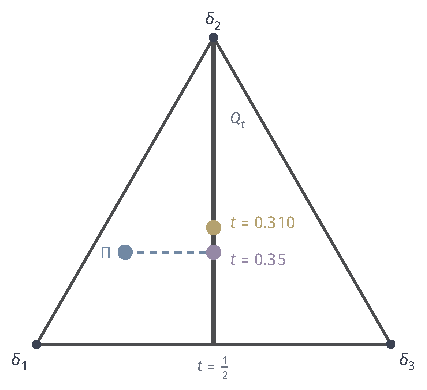
\includegraphics[width=72mm]{figures/07-probability/07-distribution-optimization/tikz/dapx-simplex-segment/figure.pdf}
 \caption{三状态概率表组成的三角形，顶点$\delta_k$是集中在状态$k$的分布，一点到三边的远近给出三个概率。蓝点是目标$\Pi=(0.6,0.3,0.1)$，深灰粗线是候选族$Q_t$（从$\delta_2$到底边中点）。黄点是按候选加权的最优解$t=0.310$，紫点是按目标加权的最优解$t=0.35$，它与$\Pi$等高，即中间状态的概率同为$0.3$。}
 \label{fig:dapx-simplex-segment}
\end{BookInlineFigure}

图~\ref{fig:dapx-simplex-segment}把这件事放在概率单纯形里：候选族是一条线段，目标在线段之外，两个方向在线段上选了不同的点。图~\ref{fig:dapx-three-point}画出两条目标曲线和三个分布的概率。两条曲线都是凸的，最低点相距$0.04$；概率图中，黄色候选把多出的概率放在中间状态，紫色候选保持中间状态与目标一致。

\begin{BookInlineFigure}
 \centering
 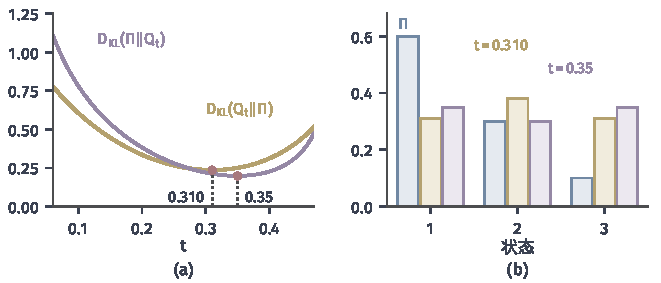
\includegraphics[width=112mm]{figures/07-probability/07-distribution-optimization/matplotlib/dapx-three-point/figure.pdf}
 \caption{三状态例子的两个方向。(a)$D_{\mathrm{KL}}(Q_t\Vert\Pi)$（黄）与$D_{\mathrm{KL}}(\Pi\Vert Q_t)$（紫）随$t$的变化，红点是最小点$t=0.310$与$t=0.35$。(b)目标$\Pi$（蓝）与两个最优候选（黄：$t=0.310$；紫：$t=0.35$）在三个状态上的概率。}
 \label{fig:dapx-three-point}
\end{BookInlineFigure}

\paragraph{择峰与覆盖}
目标有几个分离的峰而候选只有一个峰时，两个方向的差别最明显。式~\eqref{eq:dapx-bimodal}的双峰目标用高斯族逼近：按目标加权的最优解是矩匹配的$\mathcal{N}(-0.8,3.72)$，它横跨两个峰，在两峰之间目标几乎没有质量的地方放了很多概率，KL约为$0.558$；按候选加权的目标函数有两个局部最小点，分别贴住一个峰，值约为$0.356$与$1.202$，接近$-\ln0.7$与$-\ln0.3$。图~\ref{fig:dapx-bimodal-fits}(b)对每个均值$m$先把$s$取到最优，画出两个目标随$m$的变化。

\begin{BookInlineFigure}
 \centering
 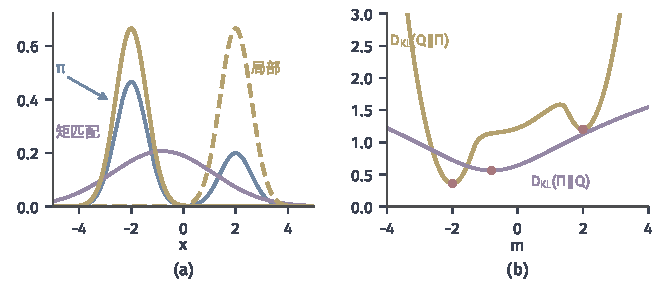
\includegraphics[width=112mm]{figures/07-probability/07-distribution-optimization/matplotlib/dapx-bimodal-fits/figure.pdf}
 \caption{用单个高斯逼近双峰目标。(a)目标（蓝）；按目标加权的最优解$\mathcal{N}(-0.8,3.72)$（紫，矩匹配）；按候选加权的两个局部最优解$\mathcal{N}(-2,0.6^{2})$（黄实线）与$\mathcal{N}(2,0.6^{2})$（黄虚线）。(b)固定均值$m$、把标准差$s$取到最优后的目标值：黄线是$D_{\mathrm{KL}}(Q\Vert\Pi)$，在$m=\pm2$附近各有一个局部最小（$0.356$与$1.202$）；紫线是$D_{\mathrm{KL}}(\Pi\Vert Q)$，只有一个最小点$m=-0.8$（$0.558$）。}
 \label{fig:dapx-bimodal-fits}
\end{BookInlineFigure}

按候选加权的方向倾向于选中目标的一个峰而忽略其他峰，称为\term{择峰}（mode seeking）；按目标加权的方向倾向于把目标所有有质量的区域都盖住，称为\term{质量覆盖}（mass covering）。这两个说法描述的是倾向，不是定理，是否出现要看目标与候选集合的具体形状。三状态例子里没有分离的峰，两个最优解都把正概率给了每个状态，按候选加权的解也没有“择”出哪一个状态，只是把概率从小概率的一端挪到了中间。能下结论的只有本节算出的这些事实：权重来自哪个分布，支持条件落在哪一边，驻点方程比较的是对数比还是比值本身。

\section{平均场逼近}
\label{sec:dapx-mean-field}

高维目标难算，往往是因为各分量纠缠在一起：求一个分量的边缘，要对其余所有分量的联合取值求和。如果候选分布让各分量独立，很多计算就拆成了一维的计算。把变量分成$m$组$\bm{x}=(x_1,\dots,x_m)$，$x_j\in\mathcal{X}_j$（每组可以是一个分量，也可以是几个分量），参考测度取各组参考测度的乘积，候选限制为
\begin{equation}
 q(\bm{x})=\prod_{j=1}^{m}q_j(x_j) ,
 \label{eq:dapx-product}
\end{equation}
其中每个因子$q_j$可以是$\mathcal{X}_j$上任意一个概率密度。用这种乘积分布逼近目标，称为\term{平均场逼近}（mean-field approximation）。名称来自统计物理：每个分量感受到的是其余分量的平均作用，下一小节的更新公式正是如此。

这里的限制只有一条：组与组之间独立。每个因子本身不限于任何参数族，可以是任意形状。所以“乘积”与“有限维参数化”是两回事：前者限制的是依赖结构，后者限制的是每个分布的形状。本节先看独立性限制本身的后果，再推导按候选加权的方向下逐个因子求最优的更新。

先处理比较简单的一个方向。按目标加权时，最优的乘积分布就是目标的边缘乘积，并且最小值正是第~\ref{chap:information-measures}章的互信息。

\begin{lemma}[正向KL下的最优乘积]
\label{lem:dapx-forward-product}
设$m=2$，目标$\Pi$有边缘$\Pi_1,\Pi_2$，且互信息有限：
\begin{equation}
 I(X_1;X_2)=D_{\mathrm{KL}}(\Pi\Vert\Pi_1\otimes\Pi_2)<\infty .
 \label{eq:dapx-mi-finite}
\end{equation}
则对任意因子$Q_1,Q_2$，
\begin{equation}
 D_{\mathrm{KL}}(\Pi\Vert Q_1\otimes Q_2)=I(X_1;X_2)+D_{\mathrm{KL}}(\Pi_1\Vert Q_1)+D_{\mathrm{KL}}(\Pi_2\Vert Q_2) .
 \label{eq:dapx-forward-product}
\end{equation}
因此最优乘积唯一，是$\Pi_1\otimes\Pi_2$，最小值是$I(X_1;X_2)$。
\end{lemma}

\begin{proof}
若$\Pi_1\not\ll Q_1$，则有集合$A$使$\Pi_1(A)>0=Q_1(A)$，于是
\[
 \Pi(A\times\mathcal{X}_2)>0=(Q_1\otimes Q_2)(A\times\mathcal{X}_2) ,
\]
两边都是$+\infty$；$\Pi_2\not\ll Q_2$同理。下设$\Pi_j\ll Q_j$，密度记为$\pi_j,q_j$。由$I<\infty$知$\Pi\ll\Pi_1\otimes\Pi_2$，于是$\Pi\ll Q_1\otimes Q_2$，并且在$\Pi$几乎处处成立
\[
 \ln\frac{\pi(x_1,x_2)}{q_1(x_1)q_2(x_2)}=\ln\frac{\pi(x_1,x_2)}{\pi_1(x_1)\pi_2(x_2)}+\ln\frac{\pi_1(x_1)}{q_1(x_1)}+\ln\frac{\pi_2(x_2)}{q_2(x_2)} .
\]
第一项的期望是有限的$I$。后两项只依赖一个变量，在$\Pi$下的期望等于在边缘下的期望，分别是$D_{\mathrm{KL}}(\Pi_j\Vert Q_j)\in[0,+\infty]$，它们的负部都可积。三项的负部都可积，期望可以逐项相加，得到式~\eqref{eq:dapx-forward-product}。后两项非负，且仅在$Q_j=\Pi_j$时为零。
\end{proof}

对上一节的概率表~\eqref{eq:dapx-table}，引理给出最优乘积是四格各$0.25$的均匀表，最小值$I(X_1;X_2)\approx0.3681$。多于两组时，同样的拆分给出最优乘积仍是各组边缘的乘积，最小值是目标与边缘乘积之间的KL。这个方向的计算需求也一目了然：需要目标的各个边缘，而求边缘往往正是困难所在。

\subsection{独立性限制的影响}
\label{sec:dapx-independence}

乘积限制会改变哪些数值特征？用一个能完整算出两个方向的例子来看。目标是均值为零、两个分量方差都是$1$、相关系数为$\rho$的二维高斯分布，
\begin{equation}
 \Pi=\mathcal{N}(\bm{0},\bm{\Sigma}),\qquad \bm{\Sigma}=\begin{bmatrix}1&\rho\\\rho&1\end{bmatrix},\qquad 0<\lvert\rho\rvert<1 .
 \label{eq:dapx-gauss-target}
\end{equation}
候选是独立的高斯分布
\[
 Q=\mathcal{N}(m_1,s_1^{2})\otimes\mathcal{N}(m_2,s_2^{2}) ,
\]
即均值为$\bm{m}=(m_1,m_2)$、协方差矩阵为$\bm{S}=\operatorname{diag}(s_1^{2},s_2^{2})$的高斯分布。需要用到精度矩阵
\[
 \bm{\Sigma}^{-1}=\frac{1}{1-\rho^{2}}\begin{bmatrix}1&-\rho\\-\rho&1\end{bmatrix},\qquad \det\bm{\Sigma}=1-\rho^{2} .
\]

\paragraph{按候选加权}
目标的对数密度是
\[
 \ln\pi(\bm{x})=-\ln(2\pi)-\tfrac12\ln(1-\rho^{2})-\tfrac12\bm{x}^{\top}\bm{\Sigma}^{-1}\bm{x} .
\]
在$Q$下，二次型的期望等于协方差部分加均值部分：
\[
 \mathbb{E}_{Q}\bigl[\bm{X}^{\top}\bm{\Sigma}^{-1}\bm{X}\bigr]=\operatorname{tr}(\bm{\Sigma}^{-1}\bm{S})+\bm{m}^{\top}\bm{\Sigma}^{-1}\bm{m}=\frac{s_1^{2}+s_2^{2}}{1-\rho^{2}}+\bm{m}^{\top}\bm{\Sigma}^{-1}\bm{m} .
\]
候选自身的对数密度期望是两个一维高斯负熵之和，$-\ln(2\pi)-\ln s_1-\ln s_2-1$。相减得
\[
 D_{\mathrm{KL}}(Q\Vert\Pi)=-\ln s_1-\ln s_2-1+\tfrac12\ln(1-\rho^{2})+\frac{s_1^{2}+s_2^{2}}{2(1-\rho^{2})}+\tfrac12\bm{m}^{\top}\bm{\Sigma}^{-1}\bm{m} .
\]

$\bm{\Sigma}^{-1}$正定，均值项在$\bm{m}=\bm{0}$时最小。对$s_1$求导并令其为零，
\[
 -\frac{1}{s_1}+\frac{s_1}{1-\rho^{2}}=0,\qquad s_1^{2}=1-\rho^{2} ,
\]
$s_2$相同。代回，最小值为
\begin{equation}
 \min_{Q}D_{\mathrm{KL}}(Q\Vert\Pi)=-\ln(1-\rho^{2})-1+\tfrac12\ln(1-\rho^{2})+1=-\tfrac12\ln(1-\rho^{2}) .
 \label{eq:dapx-gauss-reverse}
\end{equation}
最优因子的方差$1-\rho^{2}$不是目标的边缘方差$1$，而是给定另一个分量后的条件方差，也是精度矩阵对角元的倒数$1/(\bm{\Sigma}^{-1})_{1,1}$。

\paragraph{按目标加权}
由引理~\ref{lem:dapx-forward-product}，最优乘积是两个边缘$\mathcal{N}(0,1)$的乘积。最小值是高斯分布的互信息：
\[
 \begin{aligned}
 I(X_1;X_2)&=\mathbb{E}_{\Pi}\bigl[\ln\pi-\ln\pi_1-\ln\pi_2\bigr]\\
 &=-\tfrac12\ln(1-\rho^{2})+\tfrac12\,\mathbb{E}_{\Pi}\bigl[X_1^{2}+X_2^{2}-\bm{X}^{\top}\bm{\Sigma}^{-1}\bm{X}\bigr] .
 \end{aligned}
\]
$\bm{X}\sim\mathcal{N}(\bm{0},\bm{\Sigma})$时，方括号中两部分的期望相等：
\[
 \mathbb{E}\bigl[\bm{X}^{\top}\bm{\Sigma}^{-1}\bm{X}\bigr]=\operatorname{tr}(\bm{\Sigma}^{-1}\bm{\Sigma})=2,\qquad \mathbb{E}\bigl[X_1^{2}+X_2^{2}\bigr]=2 .
\]
所以
\begin{equation}
 \min_{Q}D_{\mathrm{KL}}(\Pi\Vert Q)=I(X_1;X_2)=-\tfrac12\ln(1-\rho^{2}) .
 \label{eq:dapx-gauss-forward}
\end{equation}

\paragraph{两个方向的比较}
取$\rho=0.8$。两个方向的最小值相同，都是$-\tfrac12\ln0.36\approx0.5108$，选出的分布却不同：
\[
 Q_{\mathrm{r}}=\mathcal{N}(\bm{0},0.36\,\bm{I}_2),\qquad Q_{\mathrm{f}}=\mathcal{N}(\bm{0},\bm{I}_2) .
\]
两者都把协方差删成了零，这是乘积限制本身的后果，与方向无关。区别在于分量的方差：按候选加权得到$0.36$，标准差$0.6$；按目标加权保持了$1$。图~\ref{fig:dapx-gauss-meanfield}(a)中，蓝色的目标椭圆沿对角线拉长；黄色圆被压在椭圆最窄的方向里，整个落在目标的高概率区域中；紫色虚线圆则与目标的边缘一致，但伸进了椭圆两侧目标概率很低的角落。

\begin{BookInlineFigure}
 \centering
 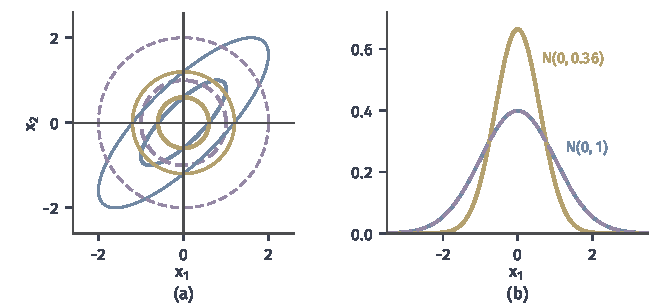
\includegraphics[width=112mm]{figures/07-probability/07-distribution-optimization/matplotlib/dapx-gauss-meanfield/figure.pdf}
 \caption{独立高斯候选逼近相关高斯目标，$\rho=0.8$。(a)等高线$\bm{x}^{\top}\bm{C}^{-1}\bm{x}=c^{2}$，$c=1,2$：目标$\bm{C}=\bm{\Sigma}$（蓝）；按候选加权的最优解$\bm{C}=0.36\,\bm{I}_2$（黄）；按目标加权的最优解$\bm{C}=\bm{I}_2$（紫色虚线）。(b)$X_1$的边缘密度：目标与按目标加权的解都是$\mathcal{N}(0,1)$（蓝线与紫色虚线重合），按候选加权的解是$\mathcal{N}(0,0.36)$（黄）。}
 \label{fig:dapx-gauss-meanfield}
\end{BookInlineFigure}

方差变小会直接影响尾概率。事件$\{\lvert X_1\rvert>1.5\}$在目标与$Q_{\mathrm{r}}$下的概率分别是
\[
 2\bigl(1-\Phi(1.5)\bigr)\approx0.134,\qquad 2\bigl(1-\Phi(1.5/0.6)\bigr)=2\bigl(1-\Phi(2.5)\bigr)\approx0.0124 ,
\]
后者小了十倍以上。所以，即使是族内最优的近似，也可能改变后续任务关心的数值特征；KL的值$0.51$本身不会告诉我们这一点。

把一个方向的最优解放到另一个方向上评价，两者都明显变差。代入上面的公式，
\[
 D_{\mathrm{KL}}(\Pi\Vert Q_{\mathrm{r}})=D_{\mathrm{KL}}(Q_{\mathrm{f}}\Vert\Pi)=\tfrac12\Bigl[\frac{2\rho^{2}}{1-\rho^{2}}+\ln(1-\rho^{2})\Bigr]\approx1.267 .
\]
图~\ref{fig:dapx-rho-curves}画出这些量随$\rho$的变化。$\rho\to\pm1$时，两个变量越来越接近同一个变量，乘积候选能做到的最好程度$-\tfrac12\ln(1-\rho^{2})$趋于无穷，按候选加权所得的方差$1-\rho^{2}$趋于零。

\begin{BookInlineFigure}
 \centering
 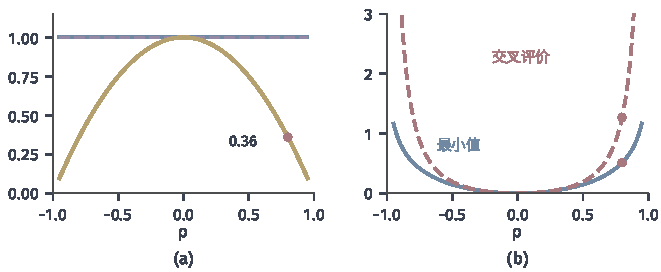
\includegraphics[width=112mm]{figures/07-probability/07-distribution-optimization/matplotlib/dapx-rho-curves/figure.pdf}
 \caption{相关系数的影响。(a)最优独立候选的分量方差：按候选加权为$1-\rho^{2}$（黄），按目标加权为$1$（紫色虚线，与目标边缘方差的蓝线重合）；红点是$\rho=0.8$时的$0.36$。(b)蓝线是两个方向共同的最小值$-\tfrac12\ln(1-\rho^{2})$；红色虚线是交叉评价，即一个方向的最优解在另一个方向上的值。}
 \label{fig:dapx-rho-curves}
\end{BookInlineFigure}

概率表~\eqref{eq:dapx-table}上也有同样的现象，只是形式不同。下一小节将求出，按候选加权的最优乘积是$q_1=q_2=(\tfrac14,\tfrac34)$或$q_1=q_2=(\tfrac34,\tfrac14)$，KL约为$0.4978$，而按目标加权的最优乘积是均匀表。前者让$Q(X_1=X_2)=\tfrac{10}{16}=0.625$，比均匀表的$0.5$更接近目标的$0.9$，代价是把边缘从$\tfrac12$改成了$\tfrac34$。两个方向在同一个乘积限制下各保留了目标的一部分特征，没有一个能全部保留。

\subsection{逐因子的坐标更新}
\label{sec:dapx-cavi}

按候选加权的方向在高斯例子里能直接求解，一般目标则不能。不过乘积结构给了一个好办法：固定其余因子，只调整一个因子，这个子问题有显式的最优解。依次对每个因子这样做，就是\term{坐标上升变分推断}（coordinate ascent variational inference），简称CAVI。“上升”指的是对$\ln Z$的变分下界~\eqref{eq:dapx-lower-bound}上升，等价于对KL下降。

\paragraph{主要思想}
固定$q_k$（$k\neq j$），把它们的乘积记为$q_{-j}$，对应的变量记为$\bm{x}_{-j}$。目标对数密度对$x_j$的依赖，在候选看来是什么样子？最自然的答案是：对其余变量按$q_{-j}$求平均。定义
\begin{equation}
 g_j(x_j)=\mathbb{E}_{q_{-j}}\bigl[\ln\widetilde{\pi}(x_j,\bm{X}_{-j})\bigr] .
 \label{eq:dapx-cavi-g}
\end{equation}
它是在“其余变量服从当前因子”的假定下，$x_j$处目标的平均对数密度。把它取指数并归一化，得到当前因子的更新：
\begin{equation}
 q_j^{\mathrm{new}}(x_j)=\frac{\exp(g_j(x_j))}{\int_{\mathcal{X}_j}\exp(g_j)\,\mathrm{d}\lambda_j} .
 \label{eq:dapx-cavi-update}
\end{equation}
下面的定理说明它恰好是子问题的唯一最优解。先在有限状态、目标处处为正的情形证明，这时所有求和都是有限和，没有可积性问题。

\begin{theorem}[逐因子最优更新]
\label{thm:dapx-cavi}
设每个$\mathcal{X}_k$是有限集，$\widetilde{\pi}(\bm{x})>0$对一切$\bm{x}$成立。固定$q_k$（$k\neq j$），按式~\eqref{eq:dapx-cavi-g}、\eqref{eq:dapx-cavi-update}定义$g_j$与$q_j^{\mathrm{new}}$。则对$\mathcal{X}_j$上任意概率$q_j$，
\begin{equation}
 D_{\mathrm{KL}}(q_j\otimes q_{-j}\Vert\Pi)=D_{\mathrm{KL}}(q_j\Vert q_j^{\mathrm{new}})+c_j ,
 \label{eq:dapx-cavi-identity}
\end{equation}
其中$c_j$只依赖$q_{-j}$与$\widetilde{\pi}$。因此$q_j^{\mathrm{new}}$是固定其余因子时唯一的最优因子。
\end{theorem}

\begin{proof}
记$Q=q_j\otimes q_{-j}$。由式~\eqref{eq:dapx-J-shift}，$D_{\mathrm{KL}}(Q\Vert\Pi)=J(Q)+\ln Z$，只需处理$J(Q)$。乘积分布的对数密度是各因子对数密度之和，所以
\[
 \mathbb{E}_{Q}[\ln q(\bm{X})]=\sum_{x_j}q_j(x_j)\ln q_j(x_j)+\sum_{k\neq j}\sum_{x_k}q_k(x_k)\ln q_k(x_k) .
\]
目标对数密度的期望先对$\bm{x}_{-j}$求和、再对$x_j$求和，由式~\eqref{eq:dapx-cavi-g}，
\[
 \mathbb{E}_{Q}[\ln\widetilde{\pi}(\bm{X})]=\sum_{x_j}q_j(x_j)\sum_{\bm{x}_{-j}}q_{-j}(\bm{x}_{-j})\ln\widetilde{\pi}(x_j,\bm{x}_{-j})=\sum_{x_j}q_j(x_j)g_j(x_j) .
\]

记$Z_j=\sum_{x_j}\exp(g_j(x_j))$，则$g_j(x_j)=\ln q_j^{\mathrm{new}}(x_j)+\ln Z_j$。两式相减，并把与$q_j$无关的项合并：
\[
 J(Q)=\sum_{x_j}q_j(x_j)\ln\frac{q_j(x_j)}{q_j^{\mathrm{new}}(x_j)}-\ln Z_j+\sum_{k\neq j}\sum_{x_k}q_k(x_k)\ln q_k(x_k) .
\]
第一项是$D_{\mathrm{KL}}(q_j\Vert q_j^{\mathrm{new}})$，其余各项不含$q_j$。加上$\ln Z$即得式~\eqref{eq:dapx-cavi-identity}，其中
\[
 c_j=-\ln Z_j+\sum_{k\neq j}\sum_{x_k}q_k(x_k)\ln q_k(x_k)+\ln Z .
\]
由Gibbs不等式，第一项非负，仅在$q_j=q_j^{\mathrm{new}}$时为零。
\end{proof}

更新公式有几处值得注意。第一，用$\widetilde{\pi}$还是$\pi$不影响结果：两者只差常数$\ln Z$，$g_j$随之平移一个常数，取指数归一化后抵消。第二，$\widetilde{\pi}(x_j,\bm{x}_{-j})$是条件密度$\pi(x_j\mid\bm{x}_{-j})$乘以一个不含$x_j$的因子，所以$q_j^{\mathrm{new}}$也正比于$\exp\bigl(\mathbb{E}_{q_{-j}}[\ln\pi(x_j\mid\bm{X}_{-j})]\bigr)$：它是目标条件分布在其余因子下的“对数平均”。这是名称中“平均场”的来源：$x_j$看到的不是其余变量的真实取值，而是它们在当前候选下的平均影响。第三，更新只用到$\ln\widetilde{\pi}$的期望，对目标只需要逐点计算未归一化密度。图~\ref{fig:dapx-factor-update}用概率表~\eqref{eq:dapx-table}演示一次更新。

\begin{BookInlineFigure}
 \centering
 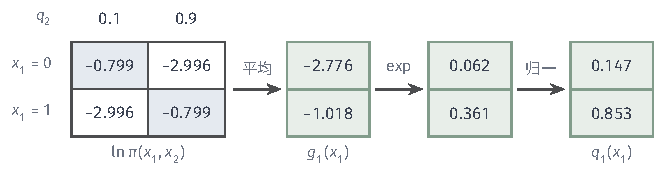
\includegraphics[width=112mm]{figures/07-probability/07-distribution-optimization/tikz/dapx-factor-update/figure.pdf}
 \caption{一次因子更新。左：目标对数概率$\ln\pi(x_1,x_2)$，列上方是当前因子$q_2=(0.1,0.9)$。按$q_2$对每一行加权平均得到$g_1(x_1)$（式~\eqref{eq:dapx-cavi-g}），取指数后归一化，得到新的$q_1=(0.147,0.853)$（式~\eqref{eq:dapx-cavi-update}）。}
 \label{fig:dapx-factor-update}
\end{BookInlineFigure}

\paragraph{高斯目标}
对式~\eqref{eq:dapx-gauss-target}的目标，记精度矩阵$\bm{\Lambda}=\bm{\Sigma}^{-1}$，取未归一化密度
\[
 \ln\widetilde{\pi}(\bm{x})=-\tfrac12\bm{x}^{\top}\bm{\Lambda}\bm{x} .
\]
固定$q_2$，记它的均值为$m_2$。展开二次型，对$X_2$求期望，只保留含$x_1$的项：
\[
 g_1(x_1)=-\tfrac12\Lambda_{1,1}x_1^{2}-\Lambda_{1,2}x_1m_2+\text{常数} .
\]
这是$x_1$的二次函数，取指数后正是高斯密度，配方得到
\[
 q_1^{\mathrm{new}}=\mathcal{N}\Bigl(-\frac{\Lambda_{1,2}}{\Lambda_{1,1}}m_2,\ \frac{1}{\Lambda_{1,1}}\Bigr)=\mathcal{N}\bigl(\rho m_2,\ 1-\rho^{2}\bigr) .
\]
因子是高斯分布这一点不是事先假定的，而是更新公式推出来的；方差$1-\rho^{2}$与上一小节一致，并且不随$q_2$改变。均值的更新是$m_1\leftarrow\rho m_2$，对第二个因子同样有$m_2\leftarrow\rho m_1$。一轮下来$m_2$乘以$\rho^{2}$，从$(m_1,m_2)=(-1.5,2)$出发，第一轮得到$m_1=1.6$，$m_2=1.28$，此后每轮缩小到$0.64$倍，收敛到唯一的最优解$\bm{m}=\bm{0}$。图~\ref{fig:dapx-cavi-gauss}画出这条阶梯形路径。

\begin{BookInlineFigure}
 \centering
 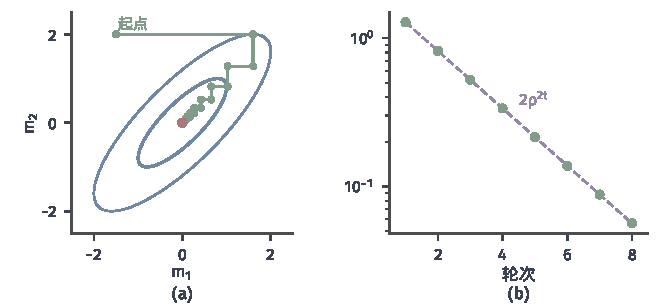
\includegraphics[width=112mm]{figures/07-probability/07-distribution-optimization/matplotlib/dapx-cavi-gauss/figure.pdf}
 \caption{高斯目标上的逐因子更新，$\rho=0.8$。(a)目标等高线（蓝）与因子均值$(m_1,m_2)$的路径（绿）：每步只沿一个坐标方向移动，起点$(-1.5,2)$，红点是最优解$\bm{0}$。(b)每轮结束时的$\lvert m_2\rvert$（绿点，对数纵轴）落在直线$2\rho^{2t}$（紫色虚线）上。}
 \label{fig:dapx-cavi-gauss}
\end{BookInlineFigure}

阶梯的每一步都很短，是因为目标沿对角线拉长：每次只能沿一个坐标轴移动，而沿坐标轴方向目标的“谷”很窄。$\lvert\rho\rvert$越接近$1$，谷越窄，每轮缩小的倍数$\rho^{2}$越接近$1$，收敛越慢。

\paragraph{一般密度}
离开有限状态，定理~\ref{thm:dapx-cavi}的推导需要以下条件，才能让每一步都是有限量的加减：
\begin{itemize}
 \item 对$\lambda_j$几乎处处的$x_j$，$\ln\widetilde{\pi}(x_j,\cdot)$在$q_{-j}$下可积，使$g_j$有定义；
 \item $0<\int\exp(g_j)\,\mathrm{d}\lambda_j<\infty$，使式~\eqref{eq:dapx-cavi-update}能够归一化；
 \item 各因子的$\mathbb{E}_{q_k}\lvert\ln q_k\rvert$有限，$\ln\widetilde{\pi}$在$q_j\otimes q_{-j}$下可积，使Fubini定理允许先对$\bm{x}_{-j}$、再对$x_j$积分。
\end{itemize}
这些条件成立时，证明中的求和换成积分，逐行照搬即可。条件不是形式上的：在高斯目标中，若当前的$q_2$是Cauchy分布，$\mathbb{E}_{q_2}[X_2]$与$\mathbb{E}_{q_2}[X_2^{2}]$都不存在，$g_1$根本没有定义。这时候选的KL也是无穷大，所以实际计算中应当从一个目标值有限的乘积出发，并逐步检查每次更新后上述积分仍然有限。

\paragraph{计算过程}
下面用概率表~\eqref{eq:dapx-table}完整走一遍。两个因子都是$\{0,1\}$上的分布，记$a=q_1(1)$，$b=q_2(1)$。

\needspace{6\baselineskip}
\paragraph{变量}
\begin{itemize}
 \item $\bm{L}\in\mathbb{R}^{2\times2}$：目标对数密度表$L_{x_1,x_2}=\ln\widetilde{\pi}(x_1,x_2)$，只读。
 \item $q_1,q_2$：两个因子，各是长度为$2$的概率向量，在原处更新；二值时只需存$a,b$。
 \item $g$：长度为$2$的工作向量，存放当前正在更新的因子的$g_j$。
 \item $D^{(t)}$：第$t$轮结束时的目标值，用于停止判断；$\varepsilon>0$为容差。
\end{itemize}

\paragraph{初始化}
读入$\bm{L}$，给出第二个因子的初值$q_2^{(0)}$，第一个因子可以任取（它会在第一步被覆盖，只用于计算初始目标值）。例中
\[
 L_{0,0}=L_{1,1}=\ln0.45\approx-0.7985,\qquad L_{0,1}=L_{1,0}=\ln0.05\approx-2.9957 ,
\]
取$q_2^{(0)}=(0.1,\ 0.9)$，$q_1^{(0)}=(0.5,\ 0.5)$，初始目标值$D^{(0)}\approx0.8789$；取$\varepsilon=10^{-4}$。

\needspace{6\baselineskip}
\paragraph{每轮更新}
第$t$轮依次执行：
\begin{enumerate}
 \item \textbf{更新第一个因子。}按式~\eqref{eq:dapx-cavi-g}对每一行用$q_2$加权：
 \[
  g(x_1)=\sum_{x_2}q_2(x_2)L_{x_1,x_2} .
 \]
 再按式~\eqref{eq:dapx-cavi-update}取指数并归一化。数值上先减去$\max g$再取指数，避免下溢。二值时归一化化简为一个logistic函数：
 \[
  a=\frac{1}{1+\exp\bigl(-(g(1)-g(0))\bigr)} .
 \]
 例中第一轮
 \[
  g(0)=0.1\cdot(-0.7985)+0.9\cdot(-2.9957)=-2.7760 ,
 \]
 \[
  g(1)=0.1\cdot(-2.9957)+0.9\cdot(-0.7985)=-1.0182 ,
 \]
 两者之差为$1.7578$，于是
 \[
  a=\frac{1}{1+\mathrm{e}^{-1.7578}}=0.8529,\qquad q_1=(0.1471,\ 0.8529) .
 \]
 这一步后目标值降到$0.5341$。

 \item \textbf{更新第二个因子。}对每一列用新的$q_1$加权：
 \[
  g(x_2)=\sum_{x_1}q_1(x_1)L_{x_1,x_2} ,
 \]
 再取指数并归一化。例中第一轮$2a-1=0.7058$，两个对数概率之差为$\ln0.45-\ln0.05=\ln9=2.1972$，
 \[
  g(1)-g(0)=(2a-1)\ln9=0.7058\cdot2.1972=1.5508 ,
 \]
 于是
 \[
  b=\frac{1}{1+\mathrm{e}^{-1.5508}}=0.8250 .
 \]

 \item \textbf{计算目标值。}乘积分布有四个格，直接求和：
 \[
  D^{(t)}=\sum_{x_1,x_2}q_1(x_1)q_2(x_2)\ln\frac{q_1(x_1)q_2(x_2)}{\pi(x_1,x_2)} .
 \]
 目标只有未归一化形式时改算$J$，停止判断只用差值，不受$\ln Z$影响。例中第一轮$D^{(1)}=0.5117$。

 \item \textbf{停止。}若$D^{(t-1)}-D^{(t)}<\varepsilon$，或已做满预定轮数，输出当前的$q_1,q_2$；否则令$t\leftarrow t+1$，回到第1步。

 例中后续各轮为
 \[
  \begin{array}{cccc}
  t & a & b & D^{(t)}\\
  2 & 0.8067 & 0.7937 & 0.50129\\
  3 & 0.7843 & 0.7772 & 0.49896\\
  4 & 0.7717 & 0.7675 & 0.49824\\
  5 & 0.7641 & 0.7614 & 0.49798\\
  6 & 0.7593 & 0.7576 & 0.49787\\
  7 & 0.7562 & 0.7551 & 0.49783
  \end{array}
 \]
 第$7$轮的下降量$4.3\times10^{-5}$小于$\varepsilon$，停止。
\end{enumerate}

最终得到$q_1\approx(0.244,\ 0.756)$，$q_2\approx(0.245,\ 0.755)$，目标值$0.49783$。继续迭代，$a,b$都趋于$\tfrac34$：二值时更新是$a=\sigma\bigl((2b-1)\ln9\bigr)$，其中$\sigma(z)=1/(1+\mathrm{e}^{-z})$，代入$b=\tfrac34$得$\sigma(\tfrac12\ln9)=\sigma(\ln3)=\tfrac34$，所以$a=b=\tfrac34$是不动点，对应的乘积分布
\[
 Q^{*}=\begin{bmatrix}\tfrac{1}{16}&\tfrac{3}{16}\\\tfrac{3}{16}&\tfrac{9}{16}\end{bmatrix},\qquad D_{\mathrm{KL}}(Q^{*}\Vert\Pi)\approx0.4978 .
\]
停止时的目标值已经与极限相差不到$10^{-4}$，因子却还差约$0.006$：目标值在最优点附近对因子的变化不敏感，用目标值的下降量作停止准则时，因子的精度要另外判断。

\paragraph{收敛与最优性}
由式~\eqref{eq:dapx-cavi-identity}，每次更新一个因子，目标值都不会增加；目标值有下界$0$，所以目标值序列收敛。这是本算法唯一无条件成立的结论。下面三件事要分开看。

第一，目标值收敛不等于因子收敛。在有限状态、各因子始终严格为正的情形，更新映射连续，每个子问题有唯一解，这类分块下降方法的极限点都是驻点；一般情形下需要的条件见\BookChapterRef{chap:block-optimization}{卷五第12章“分块优化”}。

第二，驻点不一定是最小点。从$b^{(0)}=\tfrac12$出发，第一步得到$a=\sigma(0)=\tfrac12$，之后永远停在均匀表，目标值$0.5108$。这是一个鞍点：沿$a=b$方向离开它，目标值下降。

第三，局部最优不一定是全局最优。目标值作为$(a,b)$的函数，对每个坐标单独是凸的（式~\eqref{eq:dapx-cavi-identity}右边是$q_j$的凸函数），但对两个坐标合起来不是凸的。本例有两个最小点$(\tfrac14,\tfrac14)$与$(\tfrac34,\tfrac34)$，从$b^{(0)}=0.2$出发会走到前者。这里两个最小点由对称性给出相同的值；目标不对称时，不同的局部最小点的值一般不同，迭代停在哪里取决于初值。图~\ref{fig:dapx-cavi-table}画出目标值的等高线与两条路径。

\begin{BookInlineFigure}
 \centering
 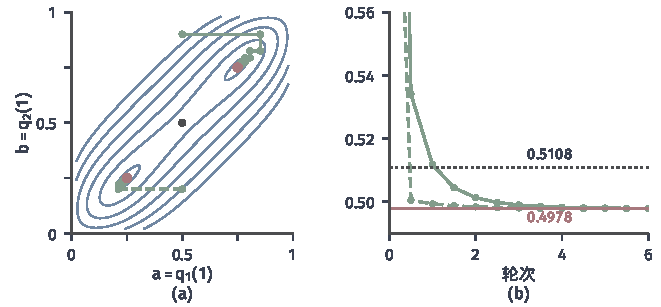
\includegraphics[width=112mm]{figures/07-probability/07-distribution-optimization/matplotlib/dapx-cavi-table/figure.pdf}
 \caption{概率表~\eqref{eq:dapx-table}上的逐因子更新。(a)乘积候选的目标值$D_{\mathrm{KL}}(q_1\otimes q_2\Vert\Pi)$关于$(a,b)$的等高线（蓝），红点是两个最小点$(\tfrac14,\tfrac14)$与$(\tfrac34,\tfrac34)$，深灰点是鞍点$(\tfrac12,\tfrac12)$；绿色实线是从$b^{(0)}=0.9$出发的路径，绿色虚线从$b^{(0)}=0.2$出发，每段折线对应一次因子更新。(b)每次因子更新后的目标值，横轴以轮计；红线是最小值$0.4978$，深灰点线是鞍点的值$0.5108$。}
 \label{fig:dapx-cavi-table}
\end{BookInlineFigure}

计算量取决于$g_j$是否容易求。若$\ln\widetilde{\pi}$是许多只涉及少数变量的项之和，例如前面的成对作用模型，那么$g_j(x_j)$只需要与$x_j$同在一项里的那些变量的因子：对二值变量，它等于$x_j$乘以$h_j+\sum_{k\neq j}J_{j,k}q_k(1)$再加常数（这里约定$J_{j,k}=J_{k,j}$），一次更新的代价与$x_j$参与的项数成正比，一轮的代价与项的总数成正比，而不是$2^{m}$。若$\ln\widetilde{\pi}$把许多变量缠在一个不可分的式子里，$g_j$本身就是一个高维期望，坐标更新也就失去了计算上的好处。

\section{参数的梯度更新}
\label{sec:dapx-gradient}

逐因子更新依赖一个前提：每个因子可以是任意分布，于是“取指数再归一化”的结果总在候选集合里。若要求因子属于某个参数族，比如规定每个因子都是高斯分布，而目标不是高斯分布，式~\eqref{eq:dapx-cavi-update}给出的$\exp(g_j)$一般不再是高斯密度，更新会跳出候选集合。又比如章首的四次方目标只有一个变量，没有可以拆分的因子。这时候选集合是一个有限维参数族，逼近问题就成了参数的优化问题。

\paragraph{参数优化问题}
设候选集合为$\{Q_{\bm{\theta}}:\bm{\theta}\in\Theta\}$，$\Theta\subset\mathbb{R}^{d}$是开集，密度$q_{\bm{\theta}}$对$\bm{\theta}$可微。按候选加权的方向，由式~\eqref{eq:dapx-J}，要最小化
\begin{equation}
 J(\bm{\theta})=\mathbb{E}_{Q_{\bm{\theta}}}\bigl[\ln q_{\bm{\theta}}(X)-\ln\widetilde{\pi}(X)\bigr] .
 \label{eq:dapx-J-theta}
\end{equation}
按目标加权的方向，在式~\eqref{eq:dapx-forward-split}成立的范围内，要最小化$-\mathbb{E}_{\Pi}[\ln q_{\bm{\theta}}(X)]$。只要目标函数可微，就可以用\BookChapterRef{chap:first-order-methods}{卷五第6章“一阶方法”}的梯度下降，
\begin{equation}
 \bm{\theta}^{(t+1)}=\bm{\theta}^{(t)}-\eta\,\nabla J\bigl(\bm{\theta}^{(t)}\bigr) ,
 \label{eq:dapx-gd}
\end{equation}
其中$\eta>0$是步长。参数还可以与乘积结构结合：每个因子取一个参数族，对所有因子的参数一起做梯度更新，或者在没有闭式解的那些因子上用梯度步代替式~\eqref{eq:dapx-cavi-update}。

两个方向的梯度对计算的要求不同。按目标加权时，在求导与期望可以交换的条件下，
\[
 \nabla_{\bm{\theta}}\bigl(-\mathbb{E}_{\Pi}[\ln q_{\bm{\theta}}(X)]\bigr)=-\mathbb{E}_{\Pi}\bigl[\nabla_{\bm{\theta}}\ln q_{\bm{\theta}}(X)\bigr] ,
\]
期望仍按目标计算；对指数族它就是$\nabla A(\bm{\theta})-\mathbb{E}_{\Pi}[\bm{T}]$，零点正是定理~\ref{thm:dapx-moment-matching}的矩匹配。按候选加权时，被积函数和求期望的分布都依赖$\bm{\theta}$，求导要同时处理两处。本节的例子里期望有闭式，可以直接求导；没有闭式时，要用样本构造梯度的随机估计，什么时候能交换求导与期望、怎样构造方差小的估计，是第~\ref{chap:expectation-gradient-estimation}章的内容，有了随机梯度后的迭代方法见\BookChapterRef{chap:stochastic-gradient-methods}{卷五第13章“随机梯度方法”}。

\paragraph{按目标加权：指数族上的凸问题}
候选是指数族时，按目标加权的目标函数在自然参数下是凸的。在式~\eqref{eq:dapx-forward-split}成立的范围内，与$\bm{\theta}$有关的部分是
\[
 -\mathbb{E}_{\Pi}[\ln q_{\bm{\theta}}(X)]=A(\bm{\theta})-\langle\bm{\theta},\mathbb{E}_{\Pi}[\bm{T}]\rangle-\mathbb{E}_{\Pi}[\ln h(X)] .
\]
第~\ref{chap:distribution-families}章证明了$A$的Hessian是$\bm{T}$的协方差矩阵，半正定，所以$A$是凸函数，再减去一个线性函数仍是凸的。凸函数的驻点就是全局最小点，梯度下降不会停在别处。

用三状态例子走几步。$Q_t$的自然参数$\theta$满足$t=\mathrm{e}^{\theta}/(1+2\mathrm{e}^{\theta})$，对数配分函数$A(\theta)=\ln(1+2\mathrm{e}^{\theta})$，$A'(\theta)=2t$，所以梯度就是矩的差：
\[
 \frac{\mathrm{d}}{\mathrm{d}\theta}D_{\mathrm{KL}}(\Pi\Vert Q_t)=2t-0.7 .
\]
取步长$\eta=2$，从$\theta^{(0)}=0$即$t=\tfrac13$出发。第一步的梯度是$\tfrac23-0.7=-0.0333$，于是
\[
 \theta^{(1)}=0+2\cdot0.0333=0.0667,\qquad t^{(1)}=0.3407 .
\]
第二步梯度为$-0.0187$，得到
\[
 \theta^{(2)}=0.104,\qquad t^{(2)}=0.3447 .
\]
在最优点附近，二阶导数$A''(\theta^{*})$等于$2t_{\mathrm{f}}(1-2t_{\mathrm{f}})=0.21$，梯度每步约乘以
\[
 1-\eta A''(\theta^{*})=1-2\cdot0.21=0.58 .
\]
第$7$步$t=0.3497$，趋于$t_{\mathrm{f}}=0.35$，对应$\theta^{*}=\ln(0.35/0.3)\approx0.154$。

按候选加权的目标函数没有这样的结构。它依赖$\bm{\theta}$的方式既通过$\ln q_{\bm{\theta}}$，也通过求期望的分布本身，在自然参数下一般不是凸的：第~\ref{sec:dapx-direction-compare}节双峰目标上的两个局部最小点就是例子。所以按候选加权时，梯度下降的结果要结合初值来解释。

\paragraph{参数化保持合法}
梯度步是在$\mathbb{R}^{d}$里走一步，走完后的参数必须仍然对应一个合法的分布。对四次方目标取候选$\mathcal{N}(m,s^{2})$，若直接以$(m,s)$为参数，由式~\eqref{eq:dapx-quartic-J}，
\[
 \frac{\partial J}{\partial s}=-\frac1s+3m^{2}s+3s^{3} .
\]
在$m=0$、$s=1.5$处它等于$-0.667+10.125=9.458$，取步长$\eta=0.2$，一步后$s=1.5-1.892<0$，不再是标准差。

改用$\omega=\ln s$作参数，$s=\mathrm{e}^{\omega}$对任何实数$\omega$都是正的，约束自动满足。由链式法则，
\[
 \frac{\partial J}{\partial\omega}=s\,\frac{\partial J}{\partial s}=1.5\cdot9.458=14.19 .
\]
同样的步长下，一步后
\[
 \omega=\ln1.5-0.2\cdot14.19=-2.43,\qquad s=\mathrm{e}^{-2.43}\approx0.088 .
\]
这个$s$合法，却走得太远，说明步长仍要另行选择；重新参数化只解决合法性。同样的办法用于其他约束：概率向量写成$p_k=\mathrm{e}^{u_k}/\sum_l\mathrm{e}^{u_l}$；协方差矩阵写成$\bm{L}\bm{L}^{\top}$，$\bm{L}$是对角元取指数的下三角矩阵，于是总是对称正定。

\paragraph{四次方目标的梯度下降}
以$(m,\omega)$为参数，把$s=\mathrm{e}^{\omega}$代入式~\eqref{eq:dapx-quartic-J}：
\[
 J(m,\omega)=-\omega-C+\tfrac14\bigl(m^{4}+6m^{2}\mathrm{e}^{2\omega}+3\mathrm{e}^{4\omega}\bigr) .
\]
分别求偏导，得到
\begin{equation}
 \frac{\partial J}{\partial m}=m^{3}+3ms^{2},\qquad \frac{\partial J}{\partial\omega}=-1+3m^{2}s^{2}+3s^{4} .
 \label{eq:dapx-quartic-grad}
\end{equation}
梯度为零要求$m(m^{2}+3s^{2})=0$，即$m=0$，再由第二式得$s^{4}=\tfrac13$，与第~\ref{sec:dapx-reverse-kl}节的结果一致。

取$\eta=0.1$，从$(m,\omega)=(1,0)$即$\mathcal{N}(1,1)$出发。第一步的梯度由式~\eqref{eq:dapx-quartic-grad}算出：
\[
 \frac{\partial J}{\partial m}=1+3=4,\qquad \frac{\partial J}{\partial\omega}=-1+3+3=5 .
\]
由式~\eqref{eq:dapx-gd}，
\[
 m^{(1)}=1-0.4=0.6,\qquad \omega^{(1)}=0-0.5=-0.5,\qquad s^{(1)}=\mathrm{e}^{-0.5}\approx0.6065 .
\]
第二步$s^{2}\approx0.3679$，$s^{4}\approx0.1353$，梯度为
\[
 \begin{aligned}
 \frac{\partial J}{\partial m}&=0.216+3\cdot0.6\cdot0.3679=0.8782,\\
 \frac{\partial J}{\partial\omega}&=-1+3\cdot0.36\cdot0.3679+3\cdot0.1353=-0.1967 ,
 \end{aligned}
\]
于是$m^{(2)}=0.5122$，$\omega^{(2)}=-0.4803$。

用$D_{\mathrm{KL}}=J+\ln Z$记录离目标的远近，前几步依次为$2.022$、$0.355$、$0.280$；第$10$步为$0.0654$，第$20$步为$0.0476$，第$40$步与族内最小值$0.0472$相同到四位小数。图~\ref{fig:dapx-gradient-path}(a)中，第一步把$\omega$拉低了很多，此后路径沿着一条弯曲的谷慢慢移向最优点。

\begin{BookInlineFigure}
 \centering
 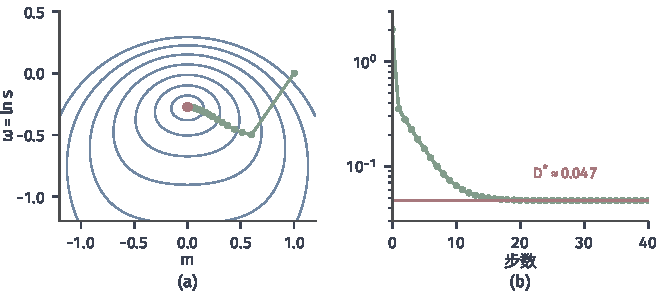
\includegraphics[width=112mm]{figures/07-probability/07-distribution-optimization/matplotlib/dapx-gradient-path/figure.pdf}
 \caption{四次方目标上高斯候选的梯度下降，参数$(m,\omega)$，$\omega=\ln s$，步长$0.1$。(a)$J(m,\omega)$的等高线（蓝）与$40$步的路径（绿），起点$(1,0)$，红点是最优解$(0,-\tfrac14\ln3)$。(b)各步的$D_{\mathrm{KL}}(Q^{(t)}\Vert\Pi)$（绿，对数纵轴），红线是族内最小值$0.0472$。}
 \label{fig:dapx-gradient-path}
\end{BookInlineFigure}

后期的收敛主要受$m$拖累。在最优点附近$s^{2}\approx3^{-1/2}$，$\partial J/\partial m\approx3s^{2}m\approx1.73\,m$，每步$m$乘以$1-0.173=0.827$，要把$m$从$0.1$降到$10^{-4}$约需$36$步。$\omega$方向的曲率不同，收敛快得多。各方向曲率不同时，同一个步长对某些方向太小、对另一些方向又可能太大，这是梯度下降在病态问题上的典型表现。在分布逼近中还有一层含义：参数空间里同样长的一步，在不同参数、不同位置引起的分布变化可能相差很大，$s$很小时改变$m$一点点，分布就几乎不再重叠。用分布本身的变化来度量步长、据此调整更新方向，是第~\ref{chap:information-geometry}章的内容。

\section{逼近误差的评价}
\label{sec:dapx-error}

算法停下来以后，手里有一个候选$\widehat{Q}$和一个算出的目标值。这个近似有多好？要回答这个问题，先要把误差的来源分开，再按后续任务选择检验的量。只看一个KL数值，既分不清误差从哪里来，也不知道它对任务意味着什么。

\paragraph{三个来源}
固定一个逼近目标，记为$\mathcal{L}(Q)$，例如$D_{\mathrm{KL}}(Q\Vert\Pi)$。设族内最优解$Q^{\dagger}\in\argmin_{Q\in\mathcal{Q}}\mathcal{L}(Q)$存在，算法输出$\widehat{Q}$，报告的目标值是$\widehat{\mathcal{L}}$。三者之间有恒等式
\begin{equation}
 \widehat{\mathcal{L}}=\underbrace{\mathcal{L}(Q^{\dagger})}_{\text{表达限制}}+\underbrace{\mathcal{L}(\widehat{Q})-\mathcal{L}(Q^{\dagger})}_{\text{优化差距}}+\underbrace{\widehat{\mathcal{L}}-\mathcal{L}(\widehat{Q})}_{\text{计算误差}} .
 \label{eq:dapx-error-parts}
\end{equation}
第一项只由目标和候选集合决定，与算法无关：候选集合里最好的分布离目标也有这么远。第二项非负，衡量算法离族内最优还差多少，它可能来自迭代步数不够，也可能来自停在了局部最优。第三项来自期望的数值计算，用样本平均估计期望时它是随机的，可正可负。图~\ref{fig:dapx-error-parts}示意了前两项。

\begin{BookInlineFigure}
 \centering
 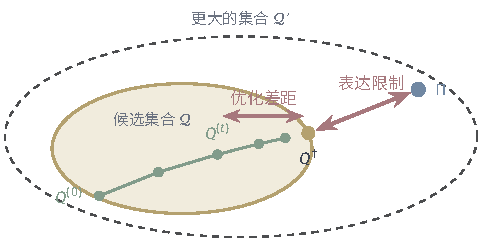
\includegraphics[width=82mm]{figures/07-probability/07-distribution-optimization/tikz/dapx-error-parts/figure.pdf}
 \caption{误差来源示意（不按比例，KL也不是几何距离）。黄色区域是候选集合$\mathcal{Q}$，蓝点是目标$\Pi$，黄点$Q^{\dagger}$是族内最优解；绿点是算法的迭代。$\Pi$到$Q^{\dagger}$的红色箭头是表达限制，迭代到$Q^{\dagger}$的红色箭头是优化差距。虚线是包含$\mathcal{Q}$的更大候选集合$\mathcal{Q}'$，它的表达限制不会更大。}
 \label{fig:dapx-error-parts}
\end{BookInlineFigure}

用四次方目标把三项都算出来。表达限制是高斯族内的最小KL，$0.0472$。第~\ref{sec:dapx-gradient}节的梯度下降做$10$步时KL为$0.0654$，优化差距是$0.0182$；做$40$步时差距已小于$10^{-4}$。计算误差来自对$J$的估计：若不用闭式~\eqref{eq:dapx-quartic-J}，而是从$Q$抽$n$个样本，用
\[
 \widehat{J}_n=\frac1n\sum_{i=1}^{n}\bigl(\ln q(X_i)-\ln\widetilde{\pi}(X_i)\bigr),\qquad X_i\sim Q\text{独立},
\]
估计$J(Q)$，它的标准差是$\sigma/\sqrt{n}$，$\sigma$是被积函数在$Q$下的标准差。在$Q^{*}$处模拟得$\sigma\approx0.409$。

$n=100$时估计的均方根误差约为$0.043$（$400$次重复，种子$727$），比第$10$步的优化差距$0.018$还大。也就是说，用$100$个样本估计目标值时，看不出第$10$步与最优解的差别；要分辨$0.018$这样的差距，需要把标准差压到它的几分之一，$n$要到几千。图~\ref{fig:dapx-mc-error}显示，误差按$n^{-1/2}$缩小，与$\sigma/\sqrt{n}$吻合。积分误差的一般理论与缩小方差的办法分别在第~\ref{chap:monte-carlo-integration-error}章和第~\ref{chap:variance-reduction}章展开。

\begin{BookInlineFigure}
 \centering
 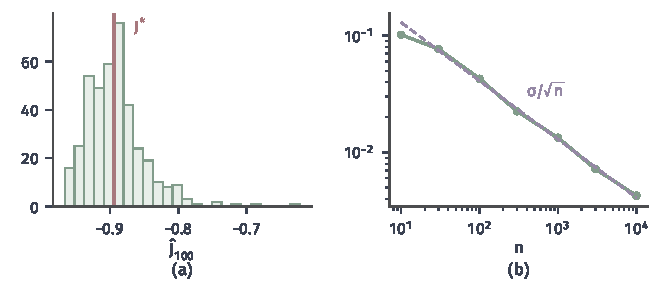
\includegraphics[width=112mm]{figures/07-probability/07-distribution-optimization/matplotlib/dapx-mc-error/figure.pdf}
 \caption{目标值的计算误差。候选为四次方目标的最优高斯$Q^{*}$，$J^{*}\approx-0.8943$。(a)$400$次独立重复中$n=100$的估计$\widehat{J}_{100}$（浅绿直方图）与真值（红线），标准差约$0.043$。(b)均方根误差随$n$的变化（绿，双对数坐标）与$\sigma/\sqrt{n}$（紫色虚线），$\sigma\approx0.409$。随机数种子为$727$。}
 \label{fig:dapx-mc-error}
\end{BookInlineFigure}

式~\eqref{eq:dapx-error-parts}还提醒一件事：当目标只有未归一化形式时，算出的是$J$而不是KL，第一项“表达限制”的大小未知，只知道$-J$是$\ln Z$的下界。比较几个候选或几个候选集合时，$J$的差就是KL的差，足以判断谁更好；要说“近似已经足够好”，则需要别的检验。

\paragraph{按任务检验}
后续任务若要用近似分布计算某些量，就应当直接检验这些量。对四次方目标，两个方向的最优高斯分别是$Q_{\mathrm{r}}=\mathcal{N}(0,0.5774)$与$Q_{\mathrm{f}}=\mathcal{N}(0,0.6760)$。比较二阶矩与四阶矩：
\[
 \begin{array}{lccc}
  & \Pi & Q_{\mathrm{r}} & Q_{\mathrm{f}}\\
 \mathbb{E}[X^{2}] & 0.676 & 0.577 & 0.676\\
 \mathbb{E}[X^{4}] & 1 & 1 & 1.371
 \end{array}
\]
目标的四阶矩由$\Gamma(5/4)=\tfrac14\Gamma(1/4)$得到：
\[
 \mathbb{E}_{\Pi}[X^{4}]=\frac{4\,\Gamma(5/4)}{\Gamma(1/4)}=1 .
\]
按目标加权的解匹配了二阶矩，这是矩匹配的直接结果，四阶矩却高估了$37\%$。按候选加权的解低估了二阶矩约$15\%$，四阶矩却恰好正确。图~\ref{fig:dapx-moment-compare}画出三个密度：目标的顶部更平、两侧下降更陡，两个高斯都无法同时匹配这两个特征。

后一个现象有原因。在候选$\mathcal{N}(0,s^{2})$中，把$X$写成$sY$，$J(s)=-\ln s-C-\mathbb{E}[\ln\widetilde{\pi}(sY)]$。对$s$求导并令其为零，再乘以$s$，得到最优尺度满足
\[
 \mathbb{E}_{Q_{\mathrm{r}}}\bigl[X\,(\ln\widetilde{\pi})'(X)\bigr]=-1 .
\]
另一方面，若$\pi$可微且$x\pi(x)\to0$（$\lvert x\rvert\to\infty$），分部积分给出
\[
 \mathbb{E}_{\Pi}\bigl[X\,(\ln\pi)'(X)\bigr]=\int x\pi'(x)\,\mathrm{d}x=-\int\pi(x)\,\mathrm{d}x=-1 .
\]
两式的左边是同一个函数$x(\ln\widetilde{\pi})'(x)$在两个分布下的期望。四次方目标中这个函数是$-x^{4}$，所以两个分布的四阶矩相同。可见，每个方向只“保留”与自己的驻点方程相关的那些平均，其余的量要单独检验。

\begin{BookInlineFigure}
 \centering
 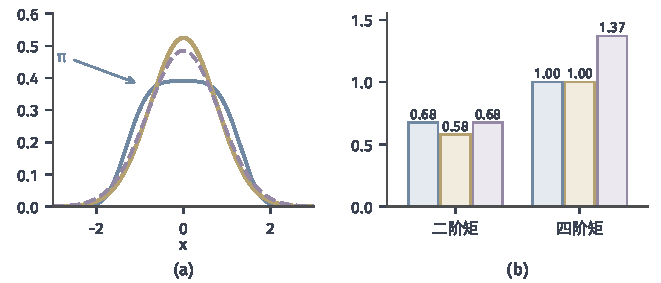
\includegraphics[width=112mm]{figures/07-probability/07-distribution-optimization/matplotlib/dapx-moment-compare/figure.pdf}
 \caption{四次方目标的两个高斯近似。(a)目标密度（蓝），按候选加权的最优解$\mathcal{N}(0,0.577)$（黄），按目标加权的最优解$\mathcal{N}(0,0.676)$（紫色虚线）。(b)三个分布的二阶矩与四阶矩，颜色同(a)。}
 \label{fig:dapx-moment-compare}
\end{BookInlineFigure}

关心事件概率时，可以用第~\ref{chap:distribution-comparison}章的Pinsker不等式$d_{\mathrm{TV}}\leq\sqrt{D_{\mathrm{KL}}/2}$。总变差是对称的，两个方向的KL都可以代入。对$Q_{\mathrm{r}}$，$D_{\mathrm{KL}}(Q_{\mathrm{r}}\Vert\Pi)\approx0.0472$给出$d_{\mathrm{TV}}\leq0.154$，数值积分得到的真值是$0.115$。对$Q_{\mathrm{f}}$，$D_{\mathrm{KL}}(\Pi\Vert Q_{\mathrm{f}})\approx0.0317$给出$d_{\mathrm{TV}}\leq0.126$，真值是$0.094$。这个上界对所有事件同时成立，但对具体的事件往往很松：$\mathbb{P}(\lvert X\rvert>1.5)$在目标下是$0.0462$，在$Q_{\mathrm{r}}$下是$0.0484$，在$Q_{\mathrm{f}}$下是$0.0681$，按候选加权的近似在这个尾概率上反而更好。

\paragraph{无界的检验函数}
若要检验的是无界函数的期望，比如矩，总变差和KL本身都不够，必须有尾部条件。第~\ref{chap:distribution-comparison}章证明了：KL要控制$g$的期望差，需要$g$在参考分布下有指数矩。反例很简单。目标为标准Cauchy分布、候选为高斯分布时，第~\ref{sec:dapx-target-candidates}节已经看到$D_{\mathrm{KL}}(Q\Vert\Pi)$有限，可是$\mathbb{E}_{\Pi}[X^{2}]=+\infty$，而每个高斯候选的二阶矩都有限。无论KL被优化到多小，用这个近似计算二阶矩都没有意义。所以，按任务检验时要先确认待求的量在目标下存在，再确认所用的比较量能控制它。

\paragraph{扩大候选集合}
若$\mathcal{Q}\subset\mathcal{Q}'$，则
\[
 \inf_{Q\in\mathcal{Q}'}\mathcal{L}(Q)\leq\inf_{Q\in\mathcal{Q}}\mathcal{L}(Q) ,
\]
因为在更大的集合里取下确界，可选的更多。这只说明式~\eqref{eq:dapx-error-parts}的第一项不会变大，并不说明实际算出的结果会变好：更大的候选集合往往带来更难的优化，第二项可能变大。

看式~\eqref{eq:dapx-bimodal}的双峰目标，目标值取$D_{\mathrm{KL}}(Q\Vert\Pi)$。单个高斯族内的最小值约为$0.356$，在左峰。两成分高斯混合族（权重、均值、方差都可变）包含目标本身，下确界为$0$。设对混合族做梯度下降，两个成分的权重都初始化为$\tfrac12$，均值和方差也取相同的值，放在右峰附近。交换两个成分不改变混合分布，所以目标值关于两组成分参数对称；在两组参数相同的点上，目标值对两组参数的偏导数也相同，每一步更新都保持两个成分相同，权重也一直是$\tfrac12$。这样的混合就是单个高斯，迭代实际上是在单个高斯族里进行，会停在右峰的局部最小点，值约为$1.202$。图~\ref{fig:dapx-larger-family}对比了这几个数。

\begin{BookInlineFigure}
 \centering
 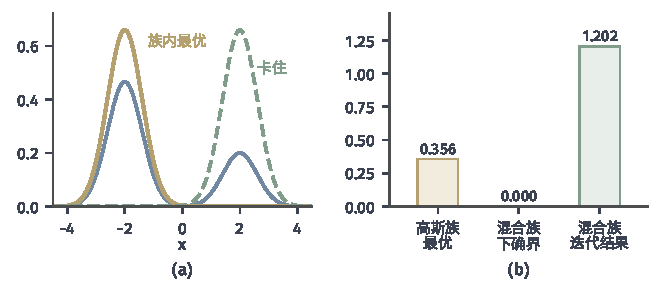
\includegraphics[width=112mm]{figures/07-probability/07-distribution-optimization/matplotlib/dapx-larger-family/figure.pdf}
 \caption{扩大候选集合不保证结果变好。(a)双峰目标（蓝）、单个高斯族内按候选加权的最优解$\mathcal{N}(-2,0.6^{2})$（黄），以及两成分完全相同地初始化在右峰附近的混合族迭代的结果（绿色虚线），它停在右峰的单个高斯上。(b)$D_{\mathrm{KL}}(Q\Vert\Pi)$：高斯族最优$0.356$，混合族下确界$0$，混合族迭代结果$1.202$。}
 \label{fig:dapx-larger-family}
\end{BookInlineFigure}

这个例子是刻意构造的，但它揭示的机制普遍存在：候选集合越大，目标函数的局部最优和对称结构往往越多。比较两个候选集合时，应当比较实际算出的结果，并报告初值与迭代设置；“族更大所以更准”只对下确界成立。

\section{本章小结}
\label{sec:dapx-summary}

章首的问题是：给定一个只能逐点计算未归一化密度的分布，怎样找一个容易计算的分布代替它。本章把这个问题拆成四个选择，每个选择都有自己的依据和代价。表~\ref{tab:dapx-summary}把它们并列。

\begin{BookInlineTable}
 \centering
 \caption{逼近问题中的四个选择。}
 \label{tab:dapx-summary}
 \begin{tabular}{lll}
  \toprule
  选择 & 选项 & 依据与代价\\
  \midrule
  候选集合 & 乘积结构 & 删去组间依赖，因子形状不限\\
   & 有限维参数族 & 限制形状，参数须保持合法\\
  KL方向 & $D_{\mathrm{KL}}(Q\Vert\Pi)$ & 需$Q\ll\Pi$；只需$\widetilde{\pi}$与$Q$下期望\\
   & $D_{\mathrm{KL}}(\Pi\Vert Q)$ & 需$\Pi\ll Q$；需$\Pi$下期望或样本\\
  求解 & 逐因子更新 & 子问题有闭式解，目标值单调下降\\
   & 参数梯度 & 适用于参数族，需梯度与步长\\
  评价 & 误差分解 & 表达限制、优化差距、计算误差\\
   & 按任务检验 & 矩、事件概率；无界函数要尾部条件\\
  \bottomrule
 \end{tabular}
\end{BookInlineTable}

候选集合决定了能保留什么。乘积候选无论怎样选择，都不能表示组间的依赖：概率表上两个变量常常相等的事实、相关高斯中的协方差都会消失。有限维参数族限制的是形状，单个高斯不能有两个峰，也不能像四次方目标那样有比高斯更轻的尾。这些损失在逼近开始之前就已确定，即式~\eqref{eq:dapx-error-parts}中的表达限制。

KL方向决定了在这些损失之间怎样取舍。按候选加权的方向惩罚候选在目标稀少处放置的质量，只要求逐点计算$\widetilde{\pi}$，因此在目标难算时最常用；它的最优解在三状态例子里给中间状态多分了概率，在相关高斯中把方差压到条件方差$1-\rho^{2}$，在双峰目标上贴住一个峰。按目标加权的方向惩罚候选对目标的覆盖不足，对指数族候选就是矩匹配，却需要目标下的期望。两个方向选出的分布一般不同，“择峰”与“覆盖”只是倾向，具体结论要按例子计算。

求解方法由候选集合的类型决定。乘积候选且因子不受限制时，每个因子的最优更新是对其余因子平均目标的对数密度，再取指数并归一化；每次更新不增加目标值，但只保证目标值收敛，可能停在鞍点或局部最优。参数族候选则用梯度下降，重新参数化保证每一步仍是合法分布，期望没有闭式时需要随机梯度。

评价时要分清误差的来源，并直接检验任务关心的量。四次方目标上，表达限制是$0.0472$，$10$步梯度下降后的优化差距是$0.018$，而用$100$个样本估计目标值的误差约为$0.043$，足以掩盖优化差距。两个方向的最优高斯分别保留了四阶矩和二阶矩，各自在另一个矩上有明显误差。扩大候选集合只降低表达限制的下确界，实际结果还取决于优化能否找到好的解。

本章假定目标分布已经给定。在统计推断中，后验分布常常正是这样一个只知道未归一化密度的目标，本章的方法可以直接用于计算它的近似；后验分布怎样由先验与数据建立、近似结果在统计上意味着什么，见\BookChapterRef{chap:parametric-statistical-inference}{卷八第1章“参数化统计推断”}。参数空间中同样长的一步引起的分布变化不同，怎样按分布的变化来度量并选择更新方向，由第~\ref{chap:information-geometry}章研究。不用近似分布、直接从目标抽样来计算期望的方法，以及这些期望估计的误差与方差，由第~\ref{chap:sample-generation}章至第~\ref{chap:expectation-gradient-estimation}章研究。

